%*************************************************************************
% A Classic Thesis Style
% An Homage to The Elements of Typographic Style
%
% Copyright (C) 2017 André Miede and Ivo Pletikosić
%
% If you like the style then I would appreciate a postcard. My address
% can be found in the file ClassicThesis.pdf. A collection of the
% postcards I received so far is available online at
% http://postcards.miede.de
%
% License:
% This program is free software; you can redistribute it and/or modify
% it under the terms of the GNU General Public License as published by
% the Free Software Foundation; either version 2 of the License, or
% (at your option) any later version.
%
% This program is distributed in the hope that it will be useful,
% but WITHOUT ANY WARRANTY; without even the implied warranty of
% MERCHANTABILITY or FITNESS FOR A PARTICULAR PURPOSE.  See the
% GNU General Public License for more details.
%
% You should have received a copy of the GNU General Public License
% along with this program; see the file COPYING.  If not, write to
% the Free Software Foundation, Inc., 59 Temple Place - Suite 330,
% Boston, MA 02111-1307, USA.
%
% PLEASE SEE ALSO THE AUTHORS' NOTE REGARDING THIS LICENSE
% IN THE DOCUMENTATION (ClassicThesis.pdf --> Chapter 1 / Chapter01.tex)
%*************************************************************************
\RequirePackage{silence} % :-\
    \WarningFilter{scrreprt}{Usage of package `titlesec'}
    %\WarningFilter{scrreprt}{Activating an ugly workaround}
    \WarningFilter{titlesec}{Non standard sectioning command detected}
\documentclass[ openright,titlepage,numbers=noenddot,headinclude,%twoside, %1headlines,% letterpaper a4paper
                footinclude=true,cleardoublepage=empty,
                BCOR=5mm,paper=a4,fontsize=11pt,%11pt,a4paper,%
                ngerman,american,%lockflag%
                ]{scrreprt}

%*************************************************************************
% Note: Make all your adjustments in here
%*************************************************************************
% ****************************************************************************************************
% hdathesis-config.tex 
% Use it at the beginning of your thesis.tex, or as a LaTeX Preamble 
% in your thesis.{tex,lyx} with % ****************************************************************************************************
% hdathesis-config.tex 
% Use it at the beginning of your thesis.tex, or as a LaTeX Preamble 
% in your thesis.{tex,lyx} with % ****************************************************************************************************
% hdathesis-config.tex 
% Use it at the beginning of your thesis.tex, or as a LaTeX Preamble 
% in your thesis.{tex,lyx} with \input{hdathesis-config}
% ****************************************************************************************************

% ****************************************************************************************************
% 1. Personal data and user ad-hoc commands
% ****************************************************************************************************
\newcommand{\myTitle}{Optimierung und Analyse dreidimensionaler Visualisierungstechniken für die effektive Darstellung von Software-Metriken\xspace}
%\newcommand{\mySubtitle}{An Homage to The Elements of Typographic Style\xspace}
\newcommand{\myDegree}{Master of Science (M.\,Sc.)\xspace}
\newcommand{\myName}{Benedikt Mehl\xspace}
\newcommand{\myId}{1121684\xspace}
\newcommand{\myProf}{Prof. Dr. Kai Renz\xspace}
%\newcommand{\myOtherProf}{Prof. Dr. Martin Girschick\xspace}
\newcommand{\myOtherProf}{--\xspace}
\newcommand{\mySupervisor}{Dr. Andreas Blunk\xspace}
\newcommand{\myFaculty}{Fachbereich Informatik\xspace}
\newcommand{\myUni}{Hochschule Darmstadt\xspace}
\newcommand{\myLocation}{Darmstadt\xspace}
\newcommand{\myTime}{\today\xspace}
\newcommand{\myVersion}{Version 0.1}

% ****************************************************************************************************
% 2. Is it a master thesis?
% ****************************************************************************************************
\PassOptionsToPackage{master}{hdathesis} % uncomment if this is a master thesis 

% ****************************************************************************************************
% 3. Does the thesis have a lock flag?
% ****************************************************************************************************
%\PassOptionsToPackage{lockflag}{hdathesis} % uncomment if this thesis has a lock flag 

% ****************************************************************************************************
% 4. Loading some handy packages
% ****************************************************************************************************
% ****************************************************************************************************
% Packages with options that might require adjustments
% ****************************************************************************************************

%\PassOptionsToPackage{ngerman,american}{babel}   % change this to your language(s)
% Spanish languages need extra options in order to work with this template
%\PassOptionsToPackage{spanish,es-lcroman}{babel}
\usepackage{babel}
\usepackage{subcaption}

\usepackage[utf8]{inputenc}

\usepackage{algorithm} 
\usepackage{algpseudocode}

\usepackage[dvipsnames]{xcolor} % Pro­vides easy driver-in­de­pen­dent ac­cess to sev­eral kinds of colors
\definecolor{tsKeyword}{RGB}{0,0,255}
\definecolor{tsString}{RGB}{163,21,21}
\definecolor{tsComment}{RGB}{0,128,0}
\definecolor{tsType}{RGB}{43,145,175}
\definecolor{tsNumber}{RGB}{128,0,128}


\usepackage{listingsutf8}
\lstdefinelanguage{json}{
    basicstyle=\ttfamily,
    morestring=[b]",
    morecomment=[l]{//},
    morecomment=[s]{/*}{*/},
    stringstyle=\color{violet},
    commentstyle=\color{green},
    showstringspaces=false
}

\lstdefinelanguage{typescript}{
    keywords={
        break, case, catch, class, const, continue, debugger, default, delete, do, else,
        enum, export, extends, false, finally, for, function, if, import, in, instanceof,
        new, null, return, super, switch, this, throw, true, try, typeof, var, void, while, with, let, await, async, static, as
    },
    keywordstyle=\color{tsKeyword}\bfseries,
    ndkeywords={
        boolean, number, string, symbol, any, never, unknown, undefined, null, object,
        interface, type, readonly, Record, Partial, Pick, Omit
    },
    ndkeywordstyle=\color{tsType}\bfseries,
    identifierstyle=\color{black},
    sensitive=true,
    comment=[l]{//},
    morecomment=[s]{/*}{*/},
    commentstyle=\color{tsComment}\itshape,
    stringstyle=\color{tsString},
    morestring=[b]',
    morestring=[b]",
    morestring=[b]`,
    numbers=left,
    numberstyle=\tiny\color{gray},
    stepnumber=1,
    numbersep=10pt,
    backgroundcolor=\color{white},
    showspaces=false,
    showstringspaces=false,
    showtabs=false,
    tabsize=2,
    breaklines=true,
    breakatwhitespace=true,
    basicstyle=\ttfamily\small,
    captionpos=b
}

\lstset{
  language=typescript,
  inputencoding=utf8,
  extendedchars=true,
  literate={ä}{{\"a}}1 {ö}{{\"o}}1 {ü}{{\"u}}1 {ß}{{\ss}}1
           {Ä}{{\"A}}1 {Ö}{{\"O}}1 {Ü}{{\"U}}1,
  basicstyle=\ttfamily\small,
  breaklines=true
}

% ****************************************************************************************************

% ****************************************************************************************************
% 1. Personal data and user ad-hoc commands
% ****************************************************************************************************
\newcommand{\myTitle}{Optimierung und Analyse dreidimensionaler Visualisierungstechniken für die effektive Darstellung von Software-Metriken\xspace}
%\newcommand{\mySubtitle}{An Homage to The Elements of Typographic Style\xspace}
\newcommand{\myDegree}{Master of Science (M.\,Sc.)\xspace}
\newcommand{\myName}{Benedikt Mehl\xspace}
\newcommand{\myId}{1121684\xspace}
\newcommand{\myProf}{Prof. Dr. Kai Renz\xspace}
%\newcommand{\myOtherProf}{Prof. Dr. Martin Girschick\xspace}
\newcommand{\myOtherProf}{--\xspace}
\newcommand{\mySupervisor}{Dr. Andreas Blunk\xspace}
\newcommand{\myFaculty}{Fachbereich Informatik\xspace}
\newcommand{\myUni}{Hochschule Darmstadt\xspace}
\newcommand{\myLocation}{Darmstadt\xspace}
\newcommand{\myTime}{\today\xspace}
\newcommand{\myVersion}{Version 0.1}

% ****************************************************************************************************
% 2. Is it a master thesis?
% ****************************************************************************************************
\PassOptionsToPackage{master}{hdathesis} % uncomment if this is a master thesis 

% ****************************************************************************************************
% 3. Does the thesis have a lock flag?
% ****************************************************************************************************
%\PassOptionsToPackage{lockflag}{hdathesis} % uncomment if this thesis has a lock flag 

% ****************************************************************************************************
% 4. Loading some handy packages
% ****************************************************************************************************
% ****************************************************************************************************
% Packages with options that might require adjustments
% ****************************************************************************************************

%\PassOptionsToPackage{ngerman,american}{babel}   % change this to your language(s)
% Spanish languages need extra options in order to work with this template
%\PassOptionsToPackage{spanish,es-lcroman}{babel}
\usepackage{babel}
\usepackage{subcaption}

\usepackage[utf8]{inputenc}

\usepackage{algorithm} 
\usepackage{algpseudocode}

\usepackage[dvipsnames]{xcolor} % Pro­vides easy driver-in­de­pen­dent ac­cess to sev­eral kinds of colors
\definecolor{tsKeyword}{RGB}{0,0,255}
\definecolor{tsString}{RGB}{163,21,21}
\definecolor{tsComment}{RGB}{0,128,0}
\definecolor{tsType}{RGB}{43,145,175}
\definecolor{tsNumber}{RGB}{128,0,128}


\usepackage{listingsutf8}
\lstdefinelanguage{json}{
    basicstyle=\ttfamily,
    morestring=[b]",
    morecomment=[l]{//},
    morecomment=[s]{/*}{*/},
    stringstyle=\color{violet},
    commentstyle=\color{green},
    showstringspaces=false
}

\lstdefinelanguage{typescript}{
    keywords={
        break, case, catch, class, const, continue, debugger, default, delete, do, else,
        enum, export, extends, false, finally, for, function, if, import, in, instanceof,
        new, null, return, super, switch, this, throw, true, try, typeof, var, void, while, with, let, await, async, static, as
    },
    keywordstyle=\color{tsKeyword}\bfseries,
    ndkeywords={
        boolean, number, string, symbol, any, never, unknown, undefined, null, object,
        interface, type, readonly, Record, Partial, Pick, Omit
    },
    ndkeywordstyle=\color{tsType}\bfseries,
    identifierstyle=\color{black},
    sensitive=true,
    comment=[l]{//},
    morecomment=[s]{/*}{*/},
    commentstyle=\color{tsComment}\itshape,
    stringstyle=\color{tsString},
    morestring=[b]',
    morestring=[b]",
    morestring=[b]`,
    numbers=left,
    numberstyle=\tiny\color{gray},
    stepnumber=1,
    numbersep=10pt,
    backgroundcolor=\color{white},
    showspaces=false,
    showstringspaces=false,
    showtabs=false,
    tabsize=2,
    breaklines=true,
    breakatwhitespace=true,
    basicstyle=\ttfamily\small,
    captionpos=b
}

\lstset{
  language=typescript,
  inputencoding=utf8,
  extendedchars=true,
  literate={ä}{{\"a}}1 {ö}{{\"o}}1 {ü}{{\"u}}1 {ß}{{\ss}}1
           {Ä}{{\"A}}1 {Ö}{{\"O}}1 {Ü}{{\"U}}1,
  basicstyle=\ttfamily\small,
  breaklines=true
}

% ****************************************************************************************************

% ****************************************************************************************************
% 1. Personal data and user ad-hoc commands
% ****************************************************************************************************
\newcommand{\myTitle}{Optimierung und Analyse dreidimensionaler Visualisierungstechniken für die effektive Darstellung von Software-Metriken\xspace}
%\newcommand{\mySubtitle}{An Homage to The Elements of Typographic Style\xspace}
\newcommand{\myDegree}{Master of Science (M.\,Sc.)\xspace}
\newcommand{\myName}{Benedikt Mehl\xspace}
\newcommand{\myId}{1121684\xspace}
\newcommand{\myProf}{Prof. Dr. Kai Renz\xspace}
%\newcommand{\myOtherProf}{Prof. Dr. Martin Girschick\xspace}
\newcommand{\myOtherProf}{--\xspace}
\newcommand{\mySupervisor}{Dr. Andreas Blunk\xspace}
\newcommand{\myFaculty}{Fachbereich Informatik\xspace}
\newcommand{\myUni}{Hochschule Darmstadt\xspace}
\newcommand{\myLocation}{Darmstadt\xspace}
\newcommand{\myTime}{\today\xspace}
\newcommand{\myVersion}{Version 0.1}

% ****************************************************************************************************
% 2. Is it a master thesis?
% ****************************************************************************************************
\PassOptionsToPackage{master}{hdathesis} % uncomment if this is a master thesis 

% ****************************************************************************************************
% 3. Does the thesis have a lock flag?
% ****************************************************************************************************
%\PassOptionsToPackage{lockflag}{hdathesis} % uncomment if this thesis has a lock flag 

% ****************************************************************************************************
% 4. Loading some handy packages
% ****************************************************************************************************
% ****************************************************************************************************
% Packages with options that might require adjustments
% ****************************************************************************************************

%\PassOptionsToPackage{ngerman,american}{babel}   % change this to your language(s)
% Spanish languages need extra options in order to work with this template
%\PassOptionsToPackage{spanish,es-lcroman}{babel}
\usepackage{babel}
\usepackage{subcaption}

\usepackage[utf8]{inputenc}

\usepackage{algorithm} 
\usepackage{algpseudocode}

\usepackage[dvipsnames]{xcolor} % Pro­vides easy driver-in­de­pen­dent ac­cess to sev­eral kinds of colors
\definecolor{tsKeyword}{RGB}{0,0,255}
\definecolor{tsString}{RGB}{163,21,21}
\definecolor{tsComment}{RGB}{0,128,0}
\definecolor{tsType}{RGB}{43,145,175}
\definecolor{tsNumber}{RGB}{128,0,128}


\usepackage{listingsutf8}
\lstdefinelanguage{json}{
    basicstyle=\ttfamily,
    morestring=[b]",
    morecomment=[l]{//},
    morecomment=[s]{/*}{*/},
    stringstyle=\color{violet},
    commentstyle=\color{green},
    showstringspaces=false
}

\lstdefinelanguage{typescript}{
    keywords={
        break, case, catch, class, const, continue, debugger, default, delete, do, else,
        enum, export, extends, false, finally, for, function, if, import, in, instanceof,
        new, null, return, super, switch, this, throw, true, try, typeof, var, void, while, with, let, await, async, static, as
    },
    keywordstyle=\color{tsKeyword}\bfseries,
    ndkeywords={
        boolean, number, string, symbol, any, never, unknown, undefined, null, object,
        interface, type, readonly, Record, Partial, Pick, Omit
    },
    ndkeywordstyle=\color{tsType}\bfseries,
    identifierstyle=\color{black},
    sensitive=true,
    comment=[l]{//},
    morecomment=[s]{/*}{*/},
    commentstyle=\color{tsComment}\itshape,
    stringstyle=\color{tsString},
    morestring=[b]',
    morestring=[b]",
    morestring=[b]`,
    numbers=left,
    numberstyle=\tiny\color{gray},
    stepnumber=1,
    numbersep=10pt,
    backgroundcolor=\color{white},
    showspaces=false,
    showstringspaces=false,
    showtabs=false,
    tabsize=2,
    breaklines=true,
    breakatwhitespace=true,
    basicstyle=\ttfamily\small,
    captionpos=b
}

\lstset{
  language=typescript,
  inputencoding=utf8,
  extendedchars=true,
  literate={ä}{{\"a}}1 {ö}{{\"o}}1 {ü}{{\"u}}1 {ß}{{\ss}}1
           {Ä}{{\"A}}1 {Ö}{{\"O}}1 {Ü}{{\"U}}1,
  basicstyle=\ttfamily\small,
  breaklines=true
}

% ****************************************************************************************************
% classicthesis-config.tex
% formerly known as loadpackages.sty, classicthesis-ldpkg.sty, and classicthesis-preamble.sty
% Use it at the beginning of your ClassicThesis.tex, or as a LaTeX Preamble
% in your ClassicThesis.{tex,lyx} with % ****************************************************************************************************
% classicthesis-config.tex
% formerly known as loadpackages.sty, classicthesis-ldpkg.sty, and classicthesis-preamble.sty
% Use it at the beginning of your ClassicThesis.tex, or as a LaTeX Preamble
% in your ClassicThesis.{tex,lyx} with % ****************************************************************************************************
% classicthesis-config.tex
% formerly known as loadpackages.sty, classicthesis-ldpkg.sty, and classicthesis-preamble.sty
% Use it at the beginning of your ClassicThesis.tex, or as a LaTeX Preamble
% in your ClassicThesis.{tex,lyx} with \input{classicthesis-config}
% ****************************************************************************************************
% If you like the classicthesis, then I would appreciate a postcard.
% My address can be found in the file ClassicThesis.pdf. A collection
% of the postcards I received so far is available online at
% http://postcards.miede.de
% ****************************************************************************************************


% ****************************************************************************************************
% 0. Set the encoding of your files. UTF-8 is the only sensible encoding nowadays. If you can't read
% äöüßáéçèê∂åëæƒÏ€ then change the encoding setting in your editor, not the line below. If your editor
% does not support utf8 use another editor!
% ****************************************************************************************************
\PassOptionsToPackage{utf8}{inputenc}
  \usepackage{inputenc}

% ****************************************************************************************************
% 1. Configure classicthesis for your needs here, e.g., remove "drafting" below
% in order to deactivate the time-stamp on the pages
% (see ClassicThesis.pdf for more information):
% ****************************************************************************************************
\PassOptionsToPackage{
  drafting=false,   % print version information on the bottom of the pages
  tocaligned=false, % the left column of the toc will be aligned (no indentation)
  dottedtoc=true,   % page numbers in ToC flushed right
  parts=true,       % use part division
  eulerchapternumbers=true, % use AMS Euler for chapter font (otherwise Palatino)
  linedheaders=false,       % chaper headers will have line above and beneath
  floatperchapter=true,     % numbering per chapter for all floats (i.e., Figure 1.1)
  listings=true,    % load listings package and setup LoL
  subfig=true,      % setup for preloaded subfig package
  eulermath=false,  % use awesome Euler fonts for mathematical formulae (only with pdfLaTeX)
  beramono=true,    % toggle a nice monospaced font (w/ bold)
  minionpro=false   % setup for minion pro font; use minion pro small caps as well (only with pdfLaTeX)
}{classicthesis}


% ****************************************************************************************************
% 2. Personal data and user ad-hoc commands
% ****************************************************************************************************
%\newcommand{\myTitle}{A Classic Thesis Style\xspace}
%\newcommand{\mySubtitle}{An Homage to The Elements of Typographic Style\xspace}
%\newcommand{\myDegree}{Doktor-Ingenieur (Dr.-Ing.)\xspace}
%\newcommand{\myName}{André Miede\xspace}
%\newcommand{\myProf}{Put name here\xspace}
%\newcommand{\myOtherProf}{Put name here\xspace}
%\newcommand{\mySupervisor}{Put name here\xspace}
%\newcommand{\myFaculty}{Put data here\xspace}
%\newcommand{\myDepartment}{Put data here\xspace}
%\newcommand{\myUni}{Put data here\xspace}
%\newcommand{\myLocation}{Saarbrücken\xspace}
%\newcommand{\myTime}{October 2017\xspace}
%\newcommand{\myVersion}{version 4.4}

% ********************************************************************
% Setup, finetuning, and useful commands
% ********************************************************************
\newcounter{dummy} % necessary for correct hyperlinks (to index, bib, etc.)
\newlength{\abcd} % for ab..z string length calculation
\providecommand{\mLyX}{L\kern-.1667em\lower.25em\hbox{Y}\kern-.125emX\@}
\newcommand{\ie}{i.\,e.}
\newcommand{\Ie}{I.\,e.}
\newcommand{\eg}{e.\,g.}
\newcommand{\Eg}{E.\,g.}
% ****************************************************************************************************


% ****************************************************************************************************
% 3. Loading some handy packages
% ****************************************************************************************************
% ********************************************************************
% Packages with options that might require adjustments
% ********************************************************************
%\PassOptionsToPackage{ngerman,american}{babel}   % change this to your language(s), main language last
% Spanish languages need extra options in order to work with this template
%\PassOptionsToPackage{spanish,es-lcroman}{babel}
\usepackage{babel}

\usepackage{csquotes}

\PassOptionsToPackage{%
  %backend=biber,bibencoding=utf8, %instead of bibtex
  backend=bibtex8,bibencoding=ascii,%
  language=auto,%
  %style=numeric-comp,%
  style=alphabetic,%
  %style=authoryear-comp, % Author 1999, 2010
  %bibstyle=authoryear,dashed=false, % dashed: substitute rep. author with ---
  sorting=nyt, % name, year, title
  maxbibnames=10, % default: 3, et al.
  %backref=true,%
  natbib=true % natbib compatibility mode (\citep and \citet still work)
}{biblatex}
  \usepackage{biblatex}

\PassOptionsToPackage{fleqn}{amsmath}       % math environments and more by the AMS
  \usepackage{amsmath}

\PassOptionsToPackage{doublespacing}{hdathesis}  % options: abbrev exam big wiwi english master
  \usepackage{hdathesis}

% ********************************************************************
% General useful packages
% ********************************************************************
\PassOptionsToPackage{T1}{fontenc} % T2A for cyrillics
  \usepackage{fontenc}
\usepackage{textcomp} % fix warning with missing font shapes
\usepackage{scrhack} % fix warnings when using KOMA with listings package
\usepackage{xspace} % to get the spacing after macros right
\usepackage{mparhack} % get marginpar right
%\usepackage{fixltx2e} % fixes some LaTeX stuff --> since 2015 in the LaTeX kernel (see below)
% \usepackage[latest]{latexrelease} % emulate newer kernel version if older is detected
\PassOptionsToPackage{printonlyused,smaller}{acronym}
  \usepackage{acronym} % nice macros for handling all acronyms in the thesis
  %\renewcommand{\bflabel}[1]{{#1}\hfill} % fix the list of acronyms --> no longer working
  %\renewcommand*{\acsfont}[1]{\textsc{#1}}
  %\renewcommand*{\aclabelfont}[1]{\acsfont{#1}}
  %\def\bflabel#1{{#1\hfill}}
  \def\bflabel#1{{\acsfont{#1}\hfill}}
  \def\aclabelfont#1{\acsfont{#1}}
% ****************************************************************************************************
%\usepackage{pgfplots} % External TikZ/PGF support (thanks to Andreas Nautsch)
%\usetikzlibrary{external}
%\tikzexternalize[mode=list and make, prefix=ext-tikz/]
% ****************************************************************************************************


% ****************************************************************************************************
% 4. Setup floats: tables, (sub)figures, and captions
% ****************************************************************************************************
\usepackage{tabularx} % better tables
  \setlength{\extrarowheight}{3pt} % increase table row height
\newcommand{\tableheadline}[1]{\multicolumn{1}{c}{\spacedlowsmallcaps{#1}}}
\newcommand{\myfloatalign}{\centering} % to be used with each float for alignment
\usepackage{caption}
% Thanks to cgnieder and Claus Lahiri
% http://tex.stackexchange.com/questions/69349/spacedlowsmallcaps-in-caption-label
% [REMOVED DUE TO OTHER PROBLEMS, SEE ISSUE #82]
%\DeclareCaptionLabelFormat{smallcaps}{\bothIfFirst{#1}{~}\MakeTextLowercase{\textsc{#2}}}
%\captionsetup{font=small,labelformat=smallcaps} % format=hang,
\captionsetup{font=small} % format=hang,
\usepackage{subfig}
% ****************************************************************************************************


% ****************************************************************************************************
% 5. Setup code listings
% ****************************************************************************************************
\usepackage{listings}
%\lstset{emph={trueIndex,root},emphstyle=\color{BlueViolet}}%\underbar} % for special keywords
\lstset{language=[LaTeX]Tex,%C++,
  morekeywords={PassOptionsToPackage,selectlanguage},
  keywordstyle=\color{RoyalBlue},%\bfseries,
  basicstyle=\small\ttfamily,
  %identifierstyle=\color{NavyBlue},
  commentstyle=\color{Green}\ttfamily,
  stringstyle=\rmfamily,
  numbers=none,%left,%
  numberstyle=\scriptsize,%\tiny
  stepnumber=5,
  numbersep=8pt,
  showstringspaces=false,
  breaklines=true,
  %frameround=ftff,
  %frame=single,
  belowcaptionskip=.75\baselineskip
  %frame=L
}
% ****************************************************************************************************


% ****************************************************************************************************
% 6. PDFLaTeX, hyperreferences, and citation backreferences
% ****************************************************************************************************
% ********************************************************************
% Using PDFLaTeX
% ********************************************************************
\PassOptionsToPackage{hyperfootnotes=false,pdfpagelabels}{hyperref}
  \usepackage{hyperref}  % backref linktocpage pagebackref
%\ifpdf
%\pdfcompresslevel=9
%\pdfadjustspacing=1
%\fi
%\PassOptionsToPackage{pdftex}{graphicx} %%%IVO: driver will be chosen automatically
  \usepackage{graphicx}


% ********************************************************************
% Hyperreferences
% ********************************************************************
\hypersetup{%
  %draft, % hyperref's draft mode, for printing see below
  colorlinks=true, linktocpage=true, pdfstartpage=3, pdfstartview=FitV,%
  % uncomment the following line if you want to have black links (e.g., for printing)
  %colorlinks=false, linktocpage=false, pdfstartpage=3, pdfstartview=FitV, pdfborder={0 0 0},%
  breaklinks=true, pdfpagemode=UseNone, pageanchor=true, pdfpagemode=UseOutlines,%
  plainpages=false, bookmarksnumbered, bookmarksopen=true, bookmarksopenlevel=1,%
  hypertexnames=true, pdfhighlight=/O,%nesting=true,%frenchlinks,%
  urlcolor=webbrown, linkcolor=RoyalBlue, citecolor=webgreen, %pagecolor=RoyalBlue,%
  %urlcolor=Black, linkcolor=Black, citecolor=Black, %pagecolor=Black,%
  pdftitle={\myTitle},%
  pdfauthor={\textcopyright\ \myName, \myUni, \myFaculty},%
  pdfsubject={},%
  pdfkeywords={},%
  pdfcreator={pdfLaTeX},%
  pdfproducer={LaTeX with hyperref and classicthesis}%
}

% ********************************************************************
% Setup autoreferences
% ********************************************************************
% There are some issues regarding autorefnames
% http://www.ureader.de/msg/136221647.aspx
% http://www.tex.ac.uk/cgi-bin/texfaq2html?label=latexwords
% you have to redefine the makros for the
% language you use, e.g., american, ngerman
% (as chosen when loading babel/AtBeginDocument)
% ********************************************************************
\makeatletter
\@ifpackageloaded{babel}%
  {%
    \addto\extrasamerican{%
      \renewcommand*{\figureautorefname}{Figure}%
      \renewcommand*{\tableautorefname}{Table}%
      \renewcommand*{\partautorefname}{Part}%
      \renewcommand*{\chapterautorefname}{Chapter}%
      \renewcommand*{\sectionautorefname}{Section}%
      \renewcommand*{\subsectionautorefname}{Section}%
      \renewcommand*{\subsubsectionautorefname}{Section}%
    }%
    \addto\extrasngerman{%
      \renewcommand*{\paragraphautorefname}{Absatz}%
      \renewcommand*{\subparagraphautorefname}{Unterabsatz}%
      \renewcommand*{\footnoteautorefname}{Fu\"snote}%
      \renewcommand*{\FancyVerbLineautorefname}{Zeile}%
      \renewcommand*{\theoremautorefname}{Theorem}%
      \renewcommand*{\appendixautorefname}{Anhang}%
      \renewcommand*{\equationautorefname}{Gleichung}%
      \renewcommand*{\itemautorefname}{Punkt}%
    }%
      % Fix to getting autorefs for subfigures right (thanks to Belinda Vogt for changing the definition)
      \providecommand{\subfigureautorefname}{\figureautorefname}%
    }{\relax}
\makeatother


% ****************************************************************************************************
% 7. Last calls before the bar closes
% ****************************************************************************************************
% ********************************************************************
% Development Stuff
% ********************************************************************
\listfiles
%\PassOptionsToPackage{l2tabu,orthodox,abort}{nag}
%  \usepackage{nag}
%\PassOptionsToPackage{warning, all}{onlyamsmath}
%  \usepackage{onlyamsmath}

% ********************************************************************
% Last, but not least...
% ********************************************************************
\usepackage{classicthesis}
% ****************************************************************************************************


% ****************************************************************************************************
% 8. Further adjustments (experimental)
% ****************************************************************************************************
% ********************************************************************
% Changing the text area
% ********************************************************************
%\areaset[current]{312pt}{761pt} % 686 (factor 2.2) + 33 head + 42 head \the\footskip
%\setlength{\marginparwidth}{7em}%
%\setlength{\marginparsep}{2em}%

% ********************************************************************
% Using different fonts
% ********************************************************************
%\usepackage[oldstylenums]{kpfonts} % oldstyle notextcomp
%\usepackage[osf]{libertine}
%\usepackage[light,condensed,math]{iwona}
%\renewcommand{\sfdefault}{iwona}
%\usepackage{lmodern} % <-- no osf support :-(
%\usepackage{cfr-lm} %
%\usepackage[urw-garamond]{mathdesign} <-- no osf support :-(
%\usepackage[default,osfigures]{opensans} % scale=0.95
%\usepackage[sfdefault]{FiraSans}
% ********************************************************************
% \usepackage[largesc,osf]{newpxtext}
% Used to fix these:
% https://bitbucket.org/amiede/classicthesis/issues/139/italics-in-pallatino-capitals-chapter
% https://bitbucket.org/amiede/classicthesis/issues/45/problema-testatine-su-classicthesis-style
% ********************************************************************
%\linespread{1.05} % a bit more for Palatino
% ****************************************************************************************************

% ****************************************************************************************************
% If you like the classicthesis, then I would appreciate a postcard.
% My address can be found in the file ClassicThesis.pdf. A collection
% of the postcards I received so far is available online at
% http://postcards.miede.de
% ****************************************************************************************************


% ****************************************************************************************************
% 0. Set the encoding of your files. UTF-8 is the only sensible encoding nowadays. If you can't read
% äöüßáéçèê∂åëæƒÏ€ then change the encoding setting in your editor, not the line below. If your editor
% does not support utf8 use another editor!
% ****************************************************************************************************
\PassOptionsToPackage{utf8}{inputenc}
  \usepackage{inputenc}

% ****************************************************************************************************
% 1. Configure classicthesis for your needs here, e.g., remove "drafting" below
% in order to deactivate the time-stamp on the pages
% (see ClassicThesis.pdf for more information):
% ****************************************************************************************************
\PassOptionsToPackage{
  drafting=false,   % print version information on the bottom of the pages
  tocaligned=false, % the left column of the toc will be aligned (no indentation)
  dottedtoc=true,   % page numbers in ToC flushed right
  parts=true,       % use part division
  eulerchapternumbers=true, % use AMS Euler for chapter font (otherwise Palatino)
  linedheaders=false,       % chaper headers will have line above and beneath
  floatperchapter=true,     % numbering per chapter for all floats (i.e., Figure 1.1)
  listings=true,    % load listings package and setup LoL
  subfig=true,      % setup for preloaded subfig package
  eulermath=false,  % use awesome Euler fonts for mathematical formulae (only with pdfLaTeX)
  beramono=true,    % toggle a nice monospaced font (w/ bold)
  minionpro=false   % setup for minion pro font; use minion pro small caps as well (only with pdfLaTeX)
}{classicthesis}


% ****************************************************************************************************
% 2. Personal data and user ad-hoc commands
% ****************************************************************************************************
%\newcommand{\myTitle}{A Classic Thesis Style\xspace}
%\newcommand{\mySubtitle}{An Homage to The Elements of Typographic Style\xspace}
%\newcommand{\myDegree}{Doktor-Ingenieur (Dr.-Ing.)\xspace}
%\newcommand{\myName}{André Miede\xspace}
%\newcommand{\myProf}{Put name here\xspace}
%\newcommand{\myOtherProf}{Put name here\xspace}
%\newcommand{\mySupervisor}{Put name here\xspace}
%\newcommand{\myFaculty}{Put data here\xspace}
%\newcommand{\myDepartment}{Put data here\xspace}
%\newcommand{\myUni}{Put data here\xspace}
%\newcommand{\myLocation}{Saarbrücken\xspace}
%\newcommand{\myTime}{October 2017\xspace}
%\newcommand{\myVersion}{version 4.4}

% ********************************************************************
% Setup, finetuning, and useful commands
% ********************************************************************
\newcounter{dummy} % necessary for correct hyperlinks (to index, bib, etc.)
\newlength{\abcd} % for ab..z string length calculation
\providecommand{\mLyX}{L\kern-.1667em\lower.25em\hbox{Y}\kern-.125emX\@}
\newcommand{\ie}{i.\,e.}
\newcommand{\Ie}{I.\,e.}
\newcommand{\eg}{e.\,g.}
\newcommand{\Eg}{E.\,g.}
% ****************************************************************************************************


% ****************************************************************************************************
% 3. Loading some handy packages
% ****************************************************************************************************
% ********************************************************************
% Packages with options that might require adjustments
% ********************************************************************
%\PassOptionsToPackage{ngerman,american}{babel}   % change this to your language(s), main language last
% Spanish languages need extra options in order to work with this template
%\PassOptionsToPackage{spanish,es-lcroman}{babel}
\usepackage{babel}

\usepackage{csquotes}

\PassOptionsToPackage{%
  %backend=biber,bibencoding=utf8, %instead of bibtex
  backend=bibtex8,bibencoding=ascii,%
  language=auto,%
  %style=numeric-comp,%
  style=alphabetic,%
  %style=authoryear-comp, % Author 1999, 2010
  %bibstyle=authoryear,dashed=false, % dashed: substitute rep. author with ---
  sorting=nyt, % name, year, title
  maxbibnames=10, % default: 3, et al.
  %backref=true,%
  natbib=true % natbib compatibility mode (\citep and \citet still work)
}{biblatex}
  \usepackage{biblatex}

\PassOptionsToPackage{fleqn}{amsmath}       % math environments and more by the AMS
  \usepackage{amsmath}

\PassOptionsToPackage{doublespacing}{hdathesis}  % options: abbrev exam big wiwi english master
  \usepackage{hdathesis}

% ********************************************************************
% General useful packages
% ********************************************************************
\PassOptionsToPackage{T1}{fontenc} % T2A for cyrillics
  \usepackage{fontenc}
\usepackage{textcomp} % fix warning with missing font shapes
\usepackage{scrhack} % fix warnings when using KOMA with listings package
\usepackage{xspace} % to get the spacing after macros right
\usepackage{mparhack} % get marginpar right
%\usepackage{fixltx2e} % fixes some LaTeX stuff --> since 2015 in the LaTeX kernel (see below)
% \usepackage[latest]{latexrelease} % emulate newer kernel version if older is detected
\PassOptionsToPackage{printonlyused,smaller}{acronym}
  \usepackage{acronym} % nice macros for handling all acronyms in the thesis
  %\renewcommand{\bflabel}[1]{{#1}\hfill} % fix the list of acronyms --> no longer working
  %\renewcommand*{\acsfont}[1]{\textsc{#1}}
  %\renewcommand*{\aclabelfont}[1]{\acsfont{#1}}
  %\def\bflabel#1{{#1\hfill}}
  \def\bflabel#1{{\acsfont{#1}\hfill}}
  \def\aclabelfont#1{\acsfont{#1}}
% ****************************************************************************************************
%\usepackage{pgfplots} % External TikZ/PGF support (thanks to Andreas Nautsch)
%\usetikzlibrary{external}
%\tikzexternalize[mode=list and make, prefix=ext-tikz/]
% ****************************************************************************************************


% ****************************************************************************************************
% 4. Setup floats: tables, (sub)figures, and captions
% ****************************************************************************************************
\usepackage{tabularx} % better tables
  \setlength{\extrarowheight}{3pt} % increase table row height
\newcommand{\tableheadline}[1]{\multicolumn{1}{c}{\spacedlowsmallcaps{#1}}}
\newcommand{\myfloatalign}{\centering} % to be used with each float for alignment
\usepackage{caption}
% Thanks to cgnieder and Claus Lahiri
% http://tex.stackexchange.com/questions/69349/spacedlowsmallcaps-in-caption-label
% [REMOVED DUE TO OTHER PROBLEMS, SEE ISSUE #82]
%\DeclareCaptionLabelFormat{smallcaps}{\bothIfFirst{#1}{~}\MakeTextLowercase{\textsc{#2}}}
%\captionsetup{font=small,labelformat=smallcaps} % format=hang,
\captionsetup{font=small} % format=hang,
\usepackage{subfig}
% ****************************************************************************************************


% ****************************************************************************************************
% 5. Setup code listings
% ****************************************************************************************************
\usepackage{listings}
%\lstset{emph={trueIndex,root},emphstyle=\color{BlueViolet}}%\underbar} % for special keywords
\lstset{language=[LaTeX]Tex,%C++,
  morekeywords={PassOptionsToPackage,selectlanguage},
  keywordstyle=\color{RoyalBlue},%\bfseries,
  basicstyle=\small\ttfamily,
  %identifierstyle=\color{NavyBlue},
  commentstyle=\color{Green}\ttfamily,
  stringstyle=\rmfamily,
  numbers=none,%left,%
  numberstyle=\scriptsize,%\tiny
  stepnumber=5,
  numbersep=8pt,
  showstringspaces=false,
  breaklines=true,
  %frameround=ftff,
  %frame=single,
  belowcaptionskip=.75\baselineskip
  %frame=L
}
% ****************************************************************************************************


% ****************************************************************************************************
% 6. PDFLaTeX, hyperreferences, and citation backreferences
% ****************************************************************************************************
% ********************************************************************
% Using PDFLaTeX
% ********************************************************************
\PassOptionsToPackage{hyperfootnotes=false,pdfpagelabels}{hyperref}
  \usepackage{hyperref}  % backref linktocpage pagebackref
%\ifpdf
%\pdfcompresslevel=9
%\pdfadjustspacing=1
%\fi
%\PassOptionsToPackage{pdftex}{graphicx} %%%IVO: driver will be chosen automatically
  \usepackage{graphicx}


% ********************************************************************
% Hyperreferences
% ********************************************************************
\hypersetup{%
  %draft, % hyperref's draft mode, for printing see below
  colorlinks=true, linktocpage=true, pdfstartpage=3, pdfstartview=FitV,%
  % uncomment the following line if you want to have black links (e.g., for printing)
  %colorlinks=false, linktocpage=false, pdfstartpage=3, pdfstartview=FitV, pdfborder={0 0 0},%
  breaklinks=true, pdfpagemode=UseNone, pageanchor=true, pdfpagemode=UseOutlines,%
  plainpages=false, bookmarksnumbered, bookmarksopen=true, bookmarksopenlevel=1,%
  hypertexnames=true, pdfhighlight=/O,%nesting=true,%frenchlinks,%
  urlcolor=webbrown, linkcolor=RoyalBlue, citecolor=webgreen, %pagecolor=RoyalBlue,%
  %urlcolor=Black, linkcolor=Black, citecolor=Black, %pagecolor=Black,%
  pdftitle={\myTitle},%
  pdfauthor={\textcopyright\ \myName, \myUni, \myFaculty},%
  pdfsubject={},%
  pdfkeywords={},%
  pdfcreator={pdfLaTeX},%
  pdfproducer={LaTeX with hyperref and classicthesis}%
}

% ********************************************************************
% Setup autoreferences
% ********************************************************************
% There are some issues regarding autorefnames
% http://www.ureader.de/msg/136221647.aspx
% http://www.tex.ac.uk/cgi-bin/texfaq2html?label=latexwords
% you have to redefine the makros for the
% language you use, e.g., american, ngerman
% (as chosen when loading babel/AtBeginDocument)
% ********************************************************************
\makeatletter
\@ifpackageloaded{babel}%
  {%
    \addto\extrasamerican{%
      \renewcommand*{\figureautorefname}{Figure}%
      \renewcommand*{\tableautorefname}{Table}%
      \renewcommand*{\partautorefname}{Part}%
      \renewcommand*{\chapterautorefname}{Chapter}%
      \renewcommand*{\sectionautorefname}{Section}%
      \renewcommand*{\subsectionautorefname}{Section}%
      \renewcommand*{\subsubsectionautorefname}{Section}%
    }%
    \addto\extrasngerman{%
      \renewcommand*{\paragraphautorefname}{Absatz}%
      \renewcommand*{\subparagraphautorefname}{Unterabsatz}%
      \renewcommand*{\footnoteautorefname}{Fu\"snote}%
      \renewcommand*{\FancyVerbLineautorefname}{Zeile}%
      \renewcommand*{\theoremautorefname}{Theorem}%
      \renewcommand*{\appendixautorefname}{Anhang}%
      \renewcommand*{\equationautorefname}{Gleichung}%
      \renewcommand*{\itemautorefname}{Punkt}%
    }%
      % Fix to getting autorefs for subfigures right (thanks to Belinda Vogt for changing the definition)
      \providecommand{\subfigureautorefname}{\figureautorefname}%
    }{\relax}
\makeatother


% ****************************************************************************************************
% 7. Last calls before the bar closes
% ****************************************************************************************************
% ********************************************************************
% Development Stuff
% ********************************************************************
\listfiles
%\PassOptionsToPackage{l2tabu,orthodox,abort}{nag}
%  \usepackage{nag}
%\PassOptionsToPackage{warning, all}{onlyamsmath}
%  \usepackage{onlyamsmath}

% ********************************************************************
% Last, but not least...
% ********************************************************************
\usepackage{classicthesis}
% ****************************************************************************************************


% ****************************************************************************************************
% 8. Further adjustments (experimental)
% ****************************************************************************************************
% ********************************************************************
% Changing the text area
% ********************************************************************
%\areaset[current]{312pt}{761pt} % 686 (factor 2.2) + 33 head + 42 head \the\footskip
%\setlength{\marginparwidth}{7em}%
%\setlength{\marginparsep}{2em}%

% ********************************************************************
% Using different fonts
% ********************************************************************
%\usepackage[oldstylenums]{kpfonts} % oldstyle notextcomp
%\usepackage[osf]{libertine}
%\usepackage[light,condensed,math]{iwona}
%\renewcommand{\sfdefault}{iwona}
%\usepackage{lmodern} % <-- no osf support :-(
%\usepackage{cfr-lm} %
%\usepackage[urw-garamond]{mathdesign} <-- no osf support :-(
%\usepackage[default,osfigures]{opensans} % scale=0.95
%\usepackage[sfdefault]{FiraSans}
% ********************************************************************
% \usepackage[largesc,osf]{newpxtext}
% Used to fix these:
% https://bitbucket.org/amiede/classicthesis/issues/139/italics-in-pallatino-capitals-chapter
% https://bitbucket.org/amiede/classicthesis/issues/45/problema-testatine-su-classicthesis-style
% ********************************************************************
%\linespread{1.05} % a bit more for Palatino
% ****************************************************************************************************

% ****************************************************************************************************
% If you like the classicthesis, then I would appreciate a postcard.
% My address can be found in the file ClassicThesis.pdf. A collection
% of the postcards I received so far is available online at
% http://postcards.miede.de
% ****************************************************************************************************


% ****************************************************************************************************
% 0. Set the encoding of your files. UTF-8 is the only sensible encoding nowadays. If you can't read
% äöüßáéçèê∂åëæƒÏ€ then change the encoding setting in your editor, not the line below. If your editor
% does not support utf8 use another editor!
% ****************************************************************************************************
\PassOptionsToPackage{utf8}{inputenc}
  \usepackage{inputenc}

% ****************************************************************************************************
% 1. Configure classicthesis for your needs here, e.g., remove "drafting" below
% in order to deactivate the time-stamp on the pages
% (see ClassicThesis.pdf for more information):
% ****************************************************************************************************
\PassOptionsToPackage{
  drafting=false,   % print version information on the bottom of the pages
  tocaligned=false, % the left column of the toc will be aligned (no indentation)
  dottedtoc=true,   % page numbers in ToC flushed right
  parts=true,       % use part division
  eulerchapternumbers=true, % use AMS Euler for chapter font (otherwise Palatino)
  linedheaders=false,       % chaper headers will have line above and beneath
  floatperchapter=true,     % numbering per chapter for all floats (i.e., Figure 1.1)
  listings=true,    % load listings package and setup LoL
  subfig=true,      % setup for preloaded subfig package
  eulermath=false,  % use awesome Euler fonts for mathematical formulae (only with pdfLaTeX)
  beramono=true,    % toggle a nice monospaced font (w/ bold)
  minionpro=false   % setup for minion pro font; use minion pro small caps as well (only with pdfLaTeX)
}{classicthesis}


% ****************************************************************************************************
% 2. Personal data and user ad-hoc commands
% ****************************************************************************************************
%\newcommand{\myTitle}{A Classic Thesis Style\xspace}
%\newcommand{\mySubtitle}{An Homage to The Elements of Typographic Style\xspace}
%\newcommand{\myDegree}{Doktor-Ingenieur (Dr.-Ing.)\xspace}
%\newcommand{\myName}{André Miede\xspace}
%\newcommand{\myProf}{Put name here\xspace}
%\newcommand{\myOtherProf}{Put name here\xspace}
%\newcommand{\mySupervisor}{Put name here\xspace}
%\newcommand{\myFaculty}{Put data here\xspace}
%\newcommand{\myDepartment}{Put data here\xspace}
%\newcommand{\myUni}{Put data here\xspace}
%\newcommand{\myLocation}{Saarbrücken\xspace}
%\newcommand{\myTime}{October 2017\xspace}
%\newcommand{\myVersion}{version 4.4}

% ********************************************************************
% Setup, finetuning, and useful commands
% ********************************************************************
\newcounter{dummy} % necessary for correct hyperlinks (to index, bib, etc.)
\newlength{\abcd} % for ab..z string length calculation
\providecommand{\mLyX}{L\kern-.1667em\lower.25em\hbox{Y}\kern-.125emX\@}
\newcommand{\ie}{i.\,e.}
\newcommand{\Ie}{I.\,e.}
\newcommand{\eg}{e.\,g.}
\newcommand{\Eg}{E.\,g.}
% ****************************************************************************************************


% ****************************************************************************************************
% 3. Loading some handy packages
% ****************************************************************************************************
% ********************************************************************
% Packages with options that might require adjustments
% ********************************************************************
%\PassOptionsToPackage{ngerman,american}{babel}   % change this to your language(s), main language last
% Spanish languages need extra options in order to work with this template
%\PassOptionsToPackage{spanish,es-lcroman}{babel}
\usepackage{babel}

\usepackage{csquotes}

\PassOptionsToPackage{%
  %backend=biber,bibencoding=utf8, %instead of bibtex
  backend=bibtex8,bibencoding=ascii,%
  language=auto,%
  %style=numeric-comp,%
  style=alphabetic,%
  %style=authoryear-comp, % Author 1999, 2010
  %bibstyle=authoryear,dashed=false, % dashed: substitute rep. author with ---
  sorting=nyt, % name, year, title
  maxbibnames=10, % default: 3, et al.
  %backref=true,%
  natbib=true % natbib compatibility mode (\citep and \citet still work)
}{biblatex}
  \usepackage{biblatex}

\PassOptionsToPackage{fleqn}{amsmath}       % math environments and more by the AMS
  \usepackage{amsmath}

\PassOptionsToPackage{doublespacing}{hdathesis}  % options: abbrev exam big wiwi english master
  \usepackage{hdathesis}

% ********************************************************************
% General useful packages
% ********************************************************************
\PassOptionsToPackage{T1}{fontenc} % T2A for cyrillics
  \usepackage{fontenc}
\usepackage{textcomp} % fix warning with missing font shapes
\usepackage{scrhack} % fix warnings when using KOMA with listings package
\usepackage{xspace} % to get the spacing after macros right
\usepackage{mparhack} % get marginpar right
%\usepackage{fixltx2e} % fixes some LaTeX stuff --> since 2015 in the LaTeX kernel (see below)
% \usepackage[latest]{latexrelease} % emulate newer kernel version if older is detected
\PassOptionsToPackage{printonlyused,smaller}{acronym}
  \usepackage{acronym} % nice macros for handling all acronyms in the thesis
  %\renewcommand{\bflabel}[1]{{#1}\hfill} % fix the list of acronyms --> no longer working
  %\renewcommand*{\acsfont}[1]{\textsc{#1}}
  %\renewcommand*{\aclabelfont}[1]{\acsfont{#1}}
  %\def\bflabel#1{{#1\hfill}}
  \def\bflabel#1{{\acsfont{#1}\hfill}}
  \def\aclabelfont#1{\acsfont{#1}}
% ****************************************************************************************************
%\usepackage{pgfplots} % External TikZ/PGF support (thanks to Andreas Nautsch)
%\usetikzlibrary{external}
%\tikzexternalize[mode=list and make, prefix=ext-tikz/]
% ****************************************************************************************************


% ****************************************************************************************************
% 4. Setup floats: tables, (sub)figures, and captions
% ****************************************************************************************************
\usepackage{tabularx} % better tables
  \setlength{\extrarowheight}{3pt} % increase table row height
\newcommand{\tableheadline}[1]{\multicolumn{1}{c}{\spacedlowsmallcaps{#1}}}
\newcommand{\myfloatalign}{\centering} % to be used with each float for alignment
\usepackage{caption}
% Thanks to cgnieder and Claus Lahiri
% http://tex.stackexchange.com/questions/69349/spacedlowsmallcaps-in-caption-label
% [REMOVED DUE TO OTHER PROBLEMS, SEE ISSUE #82]
%\DeclareCaptionLabelFormat{smallcaps}{\bothIfFirst{#1}{~}\MakeTextLowercase{\textsc{#2}}}
%\captionsetup{font=small,labelformat=smallcaps} % format=hang,
\captionsetup{font=small} % format=hang,
\usepackage{subfig}
% ****************************************************************************************************


% ****************************************************************************************************
% 5. Setup code listings
% ****************************************************************************************************
\usepackage{listings}
%\lstset{emph={trueIndex,root},emphstyle=\color{BlueViolet}}%\underbar} % for special keywords
\lstset{language=[LaTeX]Tex,%C++,
  morekeywords={PassOptionsToPackage,selectlanguage},
  keywordstyle=\color{RoyalBlue},%\bfseries,
  basicstyle=\small\ttfamily,
  %identifierstyle=\color{NavyBlue},
  commentstyle=\color{Green}\ttfamily,
  stringstyle=\rmfamily,
  numbers=none,%left,%
  numberstyle=\scriptsize,%\tiny
  stepnumber=5,
  numbersep=8pt,
  showstringspaces=false,
  breaklines=true,
  %frameround=ftff,
  %frame=single,
  belowcaptionskip=.75\baselineskip
  %frame=L
}
% ****************************************************************************************************


% ****************************************************************************************************
% 6. PDFLaTeX, hyperreferences, and citation backreferences
% ****************************************************************************************************
% ********************************************************************
% Using PDFLaTeX
% ********************************************************************
\PassOptionsToPackage{hyperfootnotes=false,pdfpagelabels}{hyperref}
  \usepackage{hyperref}  % backref linktocpage pagebackref
%\ifpdf
%\pdfcompresslevel=9
%\pdfadjustspacing=1
%\fi
%\PassOptionsToPackage{pdftex}{graphicx} %%%IVO: driver will be chosen automatically
  \usepackage{graphicx}


% ********************************************************************
% Hyperreferences
% ********************************************************************
\hypersetup{%
  %draft, % hyperref's draft mode, for printing see below
  colorlinks=true, linktocpage=true, pdfstartpage=3, pdfstartview=FitV,%
  % uncomment the following line if you want to have black links (e.g., for printing)
  %colorlinks=false, linktocpage=false, pdfstartpage=3, pdfstartview=FitV, pdfborder={0 0 0},%
  breaklinks=true, pdfpagemode=UseNone, pageanchor=true, pdfpagemode=UseOutlines,%
  plainpages=false, bookmarksnumbered, bookmarksopen=true, bookmarksopenlevel=1,%
  hypertexnames=true, pdfhighlight=/O,%nesting=true,%frenchlinks,%
  urlcolor=webbrown, linkcolor=RoyalBlue, citecolor=webgreen, %pagecolor=RoyalBlue,%
  %urlcolor=Black, linkcolor=Black, citecolor=Black, %pagecolor=Black,%
  pdftitle={\myTitle},%
  pdfauthor={\textcopyright\ \myName, \myUni, \myFaculty},%
  pdfsubject={},%
  pdfkeywords={},%
  pdfcreator={pdfLaTeX},%
  pdfproducer={LaTeX with hyperref and classicthesis}%
}

% ********************************************************************
% Setup autoreferences
% ********************************************************************
% There are some issues regarding autorefnames
% http://www.ureader.de/msg/136221647.aspx
% http://www.tex.ac.uk/cgi-bin/texfaq2html?label=latexwords
% you have to redefine the makros for the
% language you use, e.g., american, ngerman
% (as chosen when loading babel/AtBeginDocument)
% ********************************************************************
\makeatletter
\@ifpackageloaded{babel}%
  {%
    \addto\extrasamerican{%
      \renewcommand*{\figureautorefname}{Figure}%
      \renewcommand*{\tableautorefname}{Table}%
      \renewcommand*{\partautorefname}{Part}%
      \renewcommand*{\chapterautorefname}{Chapter}%
      \renewcommand*{\sectionautorefname}{Section}%
      \renewcommand*{\subsectionautorefname}{Section}%
      \renewcommand*{\subsubsectionautorefname}{Section}%
    }%
    \addto\extrasngerman{%
      \renewcommand*{\paragraphautorefname}{Absatz}%
      \renewcommand*{\subparagraphautorefname}{Unterabsatz}%
      \renewcommand*{\footnoteautorefname}{Fu\"snote}%
      \renewcommand*{\FancyVerbLineautorefname}{Zeile}%
      \renewcommand*{\theoremautorefname}{Theorem}%
      \renewcommand*{\appendixautorefname}{Anhang}%
      \renewcommand*{\equationautorefname}{Gleichung}%
      \renewcommand*{\itemautorefname}{Punkt}%
    }%
      % Fix to getting autorefs for subfigures right (thanks to Belinda Vogt for changing the definition)
      \providecommand{\subfigureautorefname}{\figureautorefname}%
    }{\relax}
\makeatother


% ****************************************************************************************************
% 7. Last calls before the bar closes
% ****************************************************************************************************
% ********************************************************************
% Development Stuff
% ********************************************************************
\listfiles
%\PassOptionsToPackage{l2tabu,orthodox,abort}{nag}
%  \usepackage{nag}
%\PassOptionsToPackage{warning, all}{onlyamsmath}
%  \usepackage{onlyamsmath}

% ********************************************************************
% Last, but not least...
% ********************************************************************
\usepackage{classicthesis}
% ****************************************************************************************************


% ****************************************************************************************************
% 8. Further adjustments (experimental)
% ****************************************************************************************************
% ********************************************************************
% Changing the text area
% ********************************************************************
%\areaset[current]{312pt}{761pt} % 686 (factor 2.2) + 33 head + 42 head \the\footskip
%\setlength{\marginparwidth}{7em}%
%\setlength{\marginparsep}{2em}%

% ********************************************************************
% Using different fonts
% ********************************************************************
%\usepackage[oldstylenums]{kpfonts} % oldstyle notextcomp
%\usepackage[osf]{libertine}
%\usepackage[light,condensed,math]{iwona}
%\renewcommand{\sfdefault}{iwona}
%\usepackage{lmodern} % <-- no osf support :-(
%\usepackage{cfr-lm} %
%\usepackage[urw-garamond]{mathdesign} <-- no osf support :-(
%\usepackage[default,osfigures]{opensans} % scale=0.95
%\usepackage[sfdefault]{FiraSans}
% ********************************************************************
% \usepackage[largesc,osf]{newpxtext}
% Used to fix these:
% https://bitbucket.org/amiede/classicthesis/issues/139/italics-in-pallatino-capitals-chapter
% https://bitbucket.org/amiede/classicthesis/issues/45/problema-testatine-su-classicthesis-style
% ********************************************************************
%\linespread{1.05} % a bit more for Palatino
% ****************************************************************************************************


%*************************************************************************
% Bibliographies
%*************************************************************************
\addbibresource{bibliography.bib}

%*************************************************************************
% Hyphenation
%*************************************************************************
%\hyphenation{put special hyphenation here}

%*************************************************************************
% GO!GO!GO! MOVE IT!
%*************************************************************************
\begin{document}
\frenchspacing
\raggedbottom
\selectlanguage{ngerman} % ngerman, american
%\renewcommand*{\bibname}{new name}
%\setbibpreamble{}
\pagenumbering{roman}
\pagestyle{plain}
%*************************************************************************
% Frontmatter
%*************************************************************************
%%*******************************************************
% Titlepage
%*******************************************************
%%%
%%% title page (german)
%%%
\thispagestyle{empty}
\pdfbookmark[0]{Titelblatt}{title}
\begin{titlepage}

  % If printed on two sides, center the title page
  \condTWOSIDE{\changetext{}{19mm}{}{19mm}{}}

  \vspace{1cm}
  \begin{center}
    \includegraphics[width=7.7cm]{gfx/logo_h-da_rot} \\ 
  \end{center}

  \begin{center}
    \vspace{0.1cm}
    \huge \textbf{\myUni}\\
    \vspace{0.4cm}
    \LARGE --~\myFaculty~--
  \end{center}

  \vfill
  \vfill

  \begin{center}
    \LARGE \textbf{\myTitle}
  \end{center} 

  \vfill
  \vfill

  \begin{center}
    \Large Abschlussarbeit zur Erlangung des akademischen Grades\\
    \vspace{0.3cm}
    \Large \myDegree
  \end{center}

  \vfill

  \begin{center}
    \Large vorgelegt von\\
    \vspace{0.3cm}
    \Large \textbf{\myName}\\
    \vspace{0.3cm}
    \normalsize Matrikelnummer: \myId
  \end{center}

  \vfill
  \vfill

  \begin{center}
    \begin{tabular}{lll}
      Referent    & : & \myProf \\
      Korreferent & : & \myOtherProf
    \end{tabular}
  \end{center} 

  % If printed on two sides, center the title page
  \condTWOSIDE{\changetext{}{-19mm}{}{-19mm}{}}

\end{titlepage}

%\include{frontbackmatter/Titleback}
%\cleardoublepage\include{frontbackmatter/Dedication}
%\cleardoublepage\include{frontbackmatter/Foreword}
%\cleardoublepage%*******************************************************
% Declaration
%*******************************************************
\refstepcounter{dummy}
\pdfbookmark[0]{Declaration}{declaration}
\chapter*{\condENGLISH{Declaration}{Erklärung}}
\thispagestyle{empty}
Ich versichere hiermit, dass ich die vorliegende Arbeit selbstständig verfasst und keine anderen als die im Literaturverzeichnis angegebenen Quellen benutzt habe.
\medskip

\noindent
Alle Stellen, die wörtlich oder sinngemäß aus veröffentlichten oder noch nicht veröffentlichten Quellen entnommen sind, sind als solche kenntlich gemacht.
\medskip

\noindent
Die Zeichnungen oder Abbildungen in dieser Arbeit sind von mir selbst erstellt worden oder mit einem entsprechenden Quellennachweis versehen.
\medskip

\noindent
Diese Arbeit ist in gleicher oder ähnlicher Form noch bei keiner anderen Prüfungsbehörde eingereicht worden. 
\bigskip

\noindent\textit{\myLocation, \myTime}

\smallskip

\begin{flushright}
    \begin{tabular}{m{5cm}}
        \\ \hline
        \centering\myName \\
    \end{tabular}
\end{flushright}

%\condLOCK{\cleardoublepage%*******************************************************
% Declaration
%*******************************************************
\refstepcounter{dummy}
\pdfbookmark[0]{Blocking Notice}{blocking notice}
\chapter*{\condENGLISH{Blocking notice}{Sperrvermerk}}
\thispagestyle{empty}

Diese Abschlussarbeit darf nur von der Referentin/ dem Referenten, der Korreferentin / dem Korreferenten sowie den vom Prüfungsausschuss dazu beauftragten Hochschulangehörigen eingesehen werden. Sie darf ohne ausdrückliche Zustimmung des Autors
weder vollständig noch auszugsweise vervielfältigt, veröffentlicht oder Dritten zugänglich gemacht werden. Die Durchführung des Kolloquiums bleibt von der Geheimhaltung unberührt. Die Geheimhaltungsverpflichtung erlischt fünf Jahre nach Einreichung automatisch.
}
%\cleardoublepage%*******************************************************
% Abstract in English
%*******************************************************
\pdfbookmark[0]{Abstract}{Abstract}


\begin{otherlanguage}{american}
	\chapter*{Abstract}
	A short summary of the contents in English of about one page. The following points should be addressed in particular:
	\begin{itemize}
		\item Motivation: Why did this work come about? Why is the topic of the work interesting (for the general public)? The motivation should be abstracted as far as possible from the specific tasks that may be given by a company.
		\item Content: What is the content of this thesis? What exactly is covered in the thesis? The methodology and working method should be briefly discussed here.
		\item Results: What are the results of this work? A brief overview of the most important results as a teaser to read the complete thesis.
	\end{itemize}
	\medskip
	
	\noindent
	BTW: A great guide by Kent Beck how to write good abstracts can be found here:
	\begin{center}
		\url{https://plg.uwaterloo.ca/~migod/research/beckOOPSLA.html}
	\end{center}
\end{otherlanguage}

%\cleardoublepage%*******************************************************
% Abstract in German
%*******************************************************
\begin{otherlanguage}{ngerman}
	\pdfbookmark[0]{Zusammenfassung}{Zusammenfassung}
	\chapter*{Zusammenfassung}
	Kurze Zusammenfassung des Inhaltes in deutscher Sprache. Ungefähr eine Seite\dots
\end{otherlanguage}

%\cleardoublepage%*******************************************************
% Publications
%*******************************************************
\pdfbookmark[0]{Publications}{publications}
\chapter*{Publications}\graffito{This is just an early --~and currently ugly~-- test!}
This might come in handy for PhD theses: some ideas and figures have appeared previously in the following publications:

%\noindent Put your publications from the thesis here. The packages \texttt{multibib} or \texttt{bibtopic} etc. can be used to handle multiple different bibliographies in your document.

\begin{refsection}[ownpubs]
    \small
    \nocite{*} % is local to to the enclosing refsection
    \printbibliography[heading=none]
\end{refsection}

\emph{Attention}: This requires a separate run of \texttt{bibtex} for your \texttt{refsection}, \eg, \texttt{ClassicThesis1-blx} for this file. You might also use \texttt{biber} as the backend for \texttt{biblatex}. See also \url{http://tex.stackexchange.com/questions/128196/problem-with-refsection}.

%\cleardoublepage%*******************************************************
% Acknowledgments
%*******************************************************
\pdfbookmark[0]{Acknowledgments}{acknowledgments}

\begin{flushright}{\slshape
    We have seen that computer programming is an art, \\
    because it applies accumulated knowledge to the world, \\
    because it requires skill and ingenuity, and especially \\
    because it produces objects of beauty.} \\ \medskip
    --- \defcitealias{knuth:1974}{Donald E. Knuth}\citetalias{knuth:1974} \citep{knuth:1974}
\end{flushright}



\bigskip

\begingroup
\let\clearpage\relax
\let\cleardoublepage\relax
\let\cleardoublepage\relax
\chapter*{Acknowledgments}
Put your acknowledgments here.

Many thanks to everybody who already sent me a postcard!

Regarding the typography and other help, many thanks go to Marco 
Kuhlmann, Philipp Lehman, Lothar Schlesier, Jim Young, Lorenzo 
Pantieri and Enrico Gregorio\footnote{Members of GuIT (Gruppo 
Italiano Utilizzatori di \TeX\ e \LaTeX )}, J\"org Sommer, 
Joachim K\"ostler, Daniel Gottschlag, Denis Aydin, Paride 
Legovini, Steffen Prochnow, Nicolas Repp, Hinrich Harms, 
Roland Winkler, Jörg Weber, Henri Menke, Claus Lahiri, 
Clemens Niederberger, Stefano Bragaglia, Jörn Hees, 
Scott Lowe, Dave Howcroft, 
and the whole \LaTeX-community for support, ideas and 
some great software.

\bigskip

\noindent\emph{Regarding \mLyX}: The \mLyX\ port was intially done by
\emph{Nicholas Mariette} in March 2009 and continued by
\emph{Ivo Pletikosi\'c} in 2011. Thank you very much for your
work and for the contributions to the original style.


\endgroup




%\cleardoublepage%*******************************************************
% Table of Contents
%*******************************************************
\pagestyle{scrheadings}
\refstepcounter{dummy}
\pdfbookmark[0]{\contentsname}{tableofcontents}
\setcounter{tocdepth}{3} % <-- 2 includes up to subsections in the ToC
\setcounter{secnumdepth}{3} % <-- 3 numbers up to subsubsections
\manualmark
\markboth{\spacedlowsmallcaps{\contentsname}}{\spacedlowsmallcaps{\contentsname}}
\tableofcontents

\cleardoublepage

%\cleardoublepage%*******************************************************
% List of Figures
%*******************************************************    
\automark[section]{chapter}
\renewcommand{\chaptermark}[1]{\markboth{\spacedlowsmallcaps{#1}}{\spacedlowsmallcaps{#1}}}
\renewcommand{\sectionmark}[1]{\markright{\thesection\enspace\spacedlowsmallcaps{#1}}}
\refstepcounter{dummy}
\pdfbookmark[0]{\listfigurename}{lof}
\listoffigures

\cleardoublepage

%\cleardoublepage%*******************************************************
% List of Tables
%*******************************************************
\automark[section]{chapter}
\renewcommand{\chaptermark}[1]{\markboth{\spacedlowsmallcaps{#1}}{\spacedlowsmallcaps{#1}}}
\renewcommand{\sectionmark}[1]{\markright{\thesection\enspace\spacedlowsmallcaps{#1}}}
\refstepcounter{dummy}
\pdfbookmark[0]{\listtablename}{lot}
\listoftables

\cleardoublepage

%\cleardoublepage%*******************************************************
% List of Listings
%*******************************************************      
\automark[section]{chapter}
\renewcommand{\chaptermark}[1]{\markboth{\spacedlowsmallcaps{#1}}{\spacedlowsmallcaps{#1}}}
\renewcommand{\sectionmark}[1]{\markright{\thesection\enspace\spacedlowsmallcaps{#1}}}
\refstepcounter{dummy}
\pdfbookmark[0]{\lstlistlistingname}{lol}
\lstlistoflistings

\cleardoublepage

%\cleardoublepage%*******************************************************
% Acronyms
%*******************************************************
\automark[section]{chapter}
\renewcommand{\chaptermark}[1]{\markboth{\spacedlowsmallcaps{#1}}{\spacedlowsmallcaps{#1}}}
\renewcommand{\sectionmark}[1]{\markright{\thesection\enspace\spacedlowsmallcaps{#1}}}
\refstepcounter{dummy}
\pdfbookmark[0]{Abk\"{u}rzungsverzeichnis}{abkuerzungsverzeichnis}
\markboth{\spacedlowsmallcaps{Abk\"{u}rzungsverzeichnis}}{\spacedlowsmallcaps{Abk\"{u}rzungsverzeichnis}}
\chapter*{Abk\"{u}rzungsverzeichnis}

% Insert your acronyms here
\begin{acronym}[UML]
  \acro{DRY}{Don't Repeat Yourself}
  \acro{API}{Application Programming Interface}
  \acro{UML}{Unified Modeling Language}
\end{acronym}

\cleardoublepage

%*************************************************************************
% Mainmatter
%*************************************************************************
\cleardoublepage
\pagestyle{scrheadings}
\pagenumbering{arabic}
% Alwas use \cleardoublepage before \part{...}.
\cleardoublepage
\part{Thesis}\label{pt:thesis}
%\include{chapters/examples/chapter01}
%\include{chapters/examples/chapter02}
%\include{chapters/examples/chapter03}
%\section{Aktueller Stand}\label{sec:aktStand}

\subsection{Generell}
Ok, erstmal ganz ganz grundlegend. 

was ist software qualität?
The ISO/IEC 25010:2011 standard [17] describes how software attributes and qualities are related. This standard decomposes software quality into eight quality characteristics:
functional suitability, performance efficiency, compatibility,
usability, reliability, security, maintainability, and portability.

ABER das ist software qualität und nicht code qualität


Was ist code qualitäts visualisierung?

für mich gibt einen einen großen unterschied zwischen code qualitäts visualisierung und code visualisierung.
Das eine soll die qualität darstellen. Das andere zb. architektur.
Das eine soll nach außen qualität zeigen und das andere eher nach innen als hilfe dienen, nicht das große ganze aus den augen zu verlieren. - grob gesagt, nur mein aktueller gedanke

In dieser arbeit geht es ausdrücklich um code qualitäts visualisierung. IMMER 

in mehr als 60\% geht es um softwre entwickler als zielgruppe (https://ieeexplore.ieee.org/abstract/document/7780158)

Was ist das ziel von code visualisierung?

Code qualitäts visualisierung soll schwach stellen und probleme im Code sichbar machen.
code visualisierung soll code gut vergleichbar machen
Es soll zeigen ob code gut oder schlecht ist.
Es soll die qualität von code aufzeigen.


Kann code qualitäts visualisierung diese ansprüche erfüllen?
so halb. Die messbarkeit von Code Qualität ist sowieso unfassbar schwer oder kaum möglich. Die Code Visualisierung kann maximal nur so gut sein wie die generelle messbarkeit von code qualität. dies ist ein komplett eigenes forschungs gebiet und hängt auch natürlich immer vom gewünschten Ziel ab.
Wir nehmen also als voraussetzung, dass das Ziel bekannt ist und die art und weise wie man die Qualität messen will auch bekannt ist.
Messwerte werden in sogenannten Metriken fest gehalten.
Bekannte und häufig genutzte metriken können sein:
lines of code
complexity
churn
coverage
issues ...
wie gesagt, ein thema für sich.


Warum braucht man also wenn man diese metriken schon hat, überhaupt noch eine visualisierung dafür?
reicht es nicht zu sagen, das sind die stellen mit schlechten werten, diese müssen angepasst werden? Oder: Diese werte sich schlecht, diese werte sind gut?
So einfach ist es oft leider nicht. 
1. zur klarstellung, was allen eigentlich schon klar ist: nur weil werte schlecht sind muss es nicht wirklich schlechter code sein
2. ist es oft wichtig auch mit personen zu kommunizieren, die keine ahnung von diesen Metriken haben. Es ist schwer zu greifen üer reine zahlen zu reden, personen wie stakeholder müssen schnell verstehen, worum es geht auch wenn sie keine ahnung von code selbst haben
3. man will sich einen generellen überblick verschaffen, in welchen bereichen sieht es gut aus, wo kann man vielleicht muster erkennen -> mit visualisierung ist es einfacher ein generelles gefühl zu entwickeln
4. übersichtlichkeit erhöhen. mit visualisierung werden die bloßen auflistungen von werten übersichtlicher


Metriken bieten außerdem niemals die qualität ab, sondern immer nur spezielle aspekte von qualität (https://ieeexplore.ieee.org/stamp/stamp.jsp?tp=&arnumber=8530132)
Eine visualisierung kann dabei helfen zugleich einzelne aspekte, aber auch ein generelles bild von qualität zu erzeugen (J. Stasko, Software visualization: Programming as a multimedia experience. MIT press, 1998.)
Das macht es vielleicht doch wieder gut, vorallem wenn zb. architekten sich einen ersten groben überblick über legacy systeme verschaffen wollen.

Es geht also nicht darum visualisierung als begründung für änderungen zu nehmen oder um entwicklern zu sagen, was und wo sie etwas besser machen müssen.
Es geht darum besonders unbeteiligten personen eine gesrächsgrundlage und einen schnellen überblick zu verschaffen. eine grundlage bieten auf der entwickler, die den code kennen mit anderen personen kommunizieren und diskutieren können. Dabei geht es nicht nur um reine funktionalität sondern auch um dinge wie UX und teilweise vielleicht auch ästethik.


Ist code visualisierung gut für entwickler?
Meine Meinung, Code Visualisierung ist nicht wirklich notwendig für entwickler, weil diese den code bereits kennen und über probleme bescheid wissen. Wenn überhaupt würden die generellen metriken wahrscheinlich ausreichen, bzw sind andere maßnahmen wie bessere Prozesse, pipelines, die automatisch metriken tracken und rückmeldung geben im alltag besser geeignet.
Für mich als entwickler wäre dann eher wieder code visualisierung und nicht code qualitäts visualisierung interessant, das ist aber wie am anfang gesagt nicht die idee hier.

\subsection{so}
Also wir gehen jetzt davon aus:
Code qualität wird mittels Metriken gemessen und wir suchen einen weg diese Metriken für (unbeteiligte) personen möglichst übersichtlich und ausagekräftig darzustellen.

\subsection{aktueller stand}
Es geht nicht um dinge wie z.b. dependency structures: https://www.ndepend.com/docs/dependency-structure-matrix-dsm


ideen von \cite{ennowulff_2021}

Wie ist der aktuelle Stand?


Welche Instrumente gibt es?
Moose - ich würde das eher bewreten für entwickler. Es werden hier verbindungen von klassen dargestellt - abhängigkeiten undco.
Another great but maybe discontinued project is Code City by Richard Wettel
https://wettel.github.io/codecity.html

"
Planung größerer Refactoring-Maßnahmen
Welche Bereiche des Codes mussten in der Vergangenheit besonders oft angepasst werden? Welche Klassen haben immer noch eine hohe Komplexität und verursachen damit hohe Wartungsaufwände? Welche Klassen besitzen einen hohen Anteil an Code-Duplikation und bergen damit das Risiko zukünftiger Fehler, falls Änderungen nicht konsistent durchgeführt werden? Mit Hilfe von SoWaCa können diese Fragen beantwortet und für alle nachvollziehbar veranschaulicht werden - vom Junior-Entwickler bis zum Manager. SoWaCa fördert damit die Kommunikation zwischen den verschiedenen Akteuren der Software-Entwickler.

Zur Retrospektive im Team
Womit hat sich das Team im letzten Sprint beschäftigt? Welche Dateien wurden am häufigsten geändert? Und in welchem Umfang? Eine Visualisierung mit Hilfe von SoWaCa hilft dem Team, sich im Rahmen der Retrospektive nochmals die wesentliche Aktivitäten des vergangenen Sprints zu vergegenwärtigen, sowie gelöste Probleme und gemachte Erfahrungen zu reflektieren.

Direkte Einblicke, automatisiert erstellt
Das letzte Architekturdiagramm ist schon drei Monate alt und berücksichtigt nicht die aktuellsten Entwicklungen? Aggregierte Kennzahlen sind gut und schön, aber wie sieht es im Detail aus? SoWaCa visualisiert voll automatisiert den aktuellen Stand der Code-Basis und ermöglicht, aus dem Überblick der gesamten Code-Basis direkt mittels "Drill-Down" auf die konkrete Code-Ebene zu springen. Damit können auf Basis aktueller Kennzahlen der Codebasis und der unmittelbaren Überprüfbarkeit fundierte Entscheidungen zur Wartung und Weiterentwicklung der Codebasis getroffen werden."
\cite{systect_2015}


code-is-beautiful: letzter commit vor 7 jahren
https://github.com/quantifiedcode/code-is-beautiful
bietet: code city, 
Sunburst (2d): im grunde ein kreis diagram, welches von  innen nach außen die ordner strukturen zeigt. die es können die größe (wie viel des kreises nimmt etwas ein) und die farbe als metric gewählt werden
Stack (2d): im grund wie das kreis diagram nur von oben nach unten


Code Radar:
https://github.com/pschild/CodeRadarVisualization
Wie code city speziell auf vergleich von versionen ausgelegt, indem man zwei karten direkt nebeneinander sehen kann
letzter commit vor 7 jahren


softvis:
vor 2 jahren
https://softvis3d.com/#/
wie code city


Ndepend:
https://www.ndepend.com/docs/treemap-visualization-of-code-metrics?cx=015095677987321916295%3Ar_17mxn8qfg&cof=FORID%3A11&q=Visualize&sa=Search#
2D
Aber interessant: hier werden die kanten dunkel eingefärbt, um die einzelnen elemente visuell zu unterscheiden


https://community.sap.com/t5/welcome-corner-blog-posts/i-have-a-dream-code-visualization/bc-p/13485189/highlight/true:
hat die idee dass gebäude wirklich echt sein könnten
ein gebäude an dem gebaut wird, wurde kürzlich geändert
alte gebäude wurden lange nicht mehr verändert
oft geänderte objekte sind nah an einem hafen oder so

ein kommentar auf deren seite:
"Playing around with these metrics seems like an easy way to identify those objects where a refactoring promises to be most beneficial, because large and complex objects that are changed often tend to introduce bugs and slow down the development process.

It also seems that this visual approach helps to promote topics like clean code within an organisation as the negative impact of such skyscraper classes becomes clearer when you look at these graphics.

I think I will take a Code City Snapshot from time to time to track how the red skyscrapers steadily turn into beautiful, clean and green suburbs.

Even without medieval buildings that can be accessed using VR, this might help a lot to navigate towards a clean code base."


https://home.uni-leipzig.de/svis/getaviz/index.php?setup=web/City%20bricks%20freemind&model=City%20bricks%20freemind&aframe=false:
auch sehr sehr nice
mit bausteinen verschiedene sachen visualisieren


https://codescene.com/product:
2d kreis diagramme

https://github.com/adamtornhill/code-maat
bietet auch einiges in 2d

Wie ist der Stand der Forschung?
overview of 3d software visualisierung: https://ieeexplore.ieee.org/document/4564449

interessant: https://opus-htw-aalen.bsz-bw.de/frontdoor/deliver/index/docId/658/file/ICCSE16-SEE.pdf

\cite{MERINO2018165}:
A systematic literature review of software visualization evaluation:
Wie kann man visualisierungen bewerten?
Hier geht es vor allem darum: "help analysts make sense of multivariate data
(Merino et al., 2015), to support programmers in comprehending the
architecture of systems (Panas et al., 2016), to help researchers analyze
version control repositories (Greene et al., 2017), and to aid developers
of software product lines"


Quality models are usually defined based on concrete measurements of software metrics (N. Fenton and J. Bieman, Software metrics: a rigorous and practical approach. CRC Press, 2014)

https://ieeexplore.ieee.org/stamp/stamp.jsp?tp=&arnumber=7332436:
4 metriken werden visualisiert: farbe, position, höhe, breite

https://ieeexplore.ieee.org/stamp/stamp.jsp?tp=&arnumber=6462737:
sehr interessant.
1. Idee unterschiedliche metriken zu stacken
2. gibt einen generelen qualitäts wert am ende heraus, erstellt aber eine grafik, die die einflüsse verschiedener klassen auf die verschiedenen metriken zeigt und die generelle bedeutung für die allgemein metrik am ende.


Was ist das? Ist das sinnvoll für mich?
To present our findings
we employ Shahin’s pre-defined classification of
visualization techniques – Graph-based, notationbased, matrix-based and metaphor-based
visualizations. 

\subsection{original square treemap algo}
– display space is used more efficiently. The number of pixels to be used for the border
is proportional to its circumference. For rectangles this number is minimal if a square
is used;
– square items are easier to detect and point at, thin rectangles clutter up and give rise
to aliasing errors;
– comparison of the size of rectangles is easier when their aspect ratios are similar;
– the accuracy of the presentation is improved. A rectangle with a prescribed width of,
say, 300 pixels, can only present sizes in coarse steps.



\section{Grundlagen} \label{sec:Grundlagen}

\subsection{Software-Qualitätsmetriken} \label{sec:SoftwareQualitaetsmetriken}
Qualitätsmetriken sind Kennzahlen, die zur Bewertung der Qualität verwendet werden. Sie sind ein wichtiges Werkzeug zur Analyse und Verbesserung jeglicher Dinge. Im grunde sind metriken einfach nur messungen, die eine bestimmte Aussagekraft haben. OFt ist es nicht möglich eine Metrik zu identifizieren, die eine vollumfängliche aussage über etwas trifft. Oft ist es notwenig verschiedene metriken im zusammenspiel miteinander zu betrachten, um ein verständis für aspekte zu erhalten. 

Dies gilt auch für Software-Qualitätsmetriken: \enquote{Eine Softwarequalitätsmetrik ist eine Funktion, die eine Software-Einheit in einen Zahlenwert abbildet, welcher als Erfüllungsgrad einer Qualitätseigenschaft der Software-Einheit interpretierbar ist.}\cite{def_qual_metric}

Es ist nicht möglich eine einzige Metrik zu finden, die eine vollumfängliche aussage über die Qualität einer Software trifft - was ist schon gute Software? Wann ist software gut? SEblst wenn man als Ziel von software definieren würde, dass sie fehlerfrei ist, wäre es nicht möglich eine einzige Metrik zu finden, die dies beschreibt. Wann ist eine software fehlerfrei? Ist sie fehlerfrei, wenn sie keine Bugs hat? Wenn sie keine Bugs hat, aber trotzdem nicht benutzbar ist, ist sie dann fehlerfrei?

Dieser Eigenschaft macht es notwendig verschiedene Metriken im zusammenspiel zu betrachten und sich einen übersblick über die Indizien zu verschaffen, die auf eine gute oder schlechte Qualität hinweisen.
Die besonderheit bei Software-Qualitätsmetriken im vergleich zu anderen Metriken mag sein, dass die Daten hierarchisch strukturiert sind. Meist wird dies auf die orderner und datei-struktur abgebildet. So werden die Metriken in der Regel auf der Ebene der einzelnen Dateien ermittelt und dann auf die Ordner-Ebene aggregiert, wodurch eine hierarchische Baumstruktur entsteht. 

Software-Qualitätsmetriken werden meist auf Software-Einheiten angewendet. Also z.B. auf Dateien des Quellcodes, auf Module oder auf Klassen. Diese Software-Einheiten sind in der Regel hierarchisch strukturiert. Auch die im folgenden vorgesllten ansätze zur Visualisierung von hierarchischen Daten sind nicht speziell für Software-Qualitätsmetriken gedacht, sondern stellen allgemeine Ansätze dar. Ich behaupte, dass die Sturktur von Software gemeinsamkeiten hat, zB. ein ordner hat nicht mehr als 20 Kinder, was interessante annahmen darstellt, die eventuell in die visualierungs algorithmen verbessernd einfließen können.  

\subsection{Software-Visualisierung} \label{sec:SoftwareVisualisierung} 

• Tasks – why is the visualization needed?
• Audience – who will use the visualization?
• Target – what is the data source to represent?
• Representation – how to represent it?
• Medium – where to represent the visualization?
\cite[2]{3dsoftwareMarcus}

\subsection{3D-Software Visualisierung} \label{sec:3DSoftwareVisualisierung}   
Warum 3D? Ist es nicht ausreichend software-qualität einfach als zahlenwerte darzustellen oder zumindest in 2D darzustellen?
wie in Abschnitt \ref{sec:Ziel} aufgezeigt, wollen wir software qualität auch für nicht-software-entwickler greifbar machen, einfache werte sind dafür nicht ausreichend.
\begin{quote}
Despite the proven usefulness of 2D visualizations, they do not allow the viewer to be immersed in a visualization, and the feeling is that we are looking at things from "outside". 3D visualizations on the other hand provide the potential to create such an immersive experience... \cite[1]{codeCity1}
\end{quote}
2D visualisierung bietet zwar bestimmt einen guten überblick, aber macht die software nicht wirklich greifbar. 

Die Idee Software in 3D darzustellen ist nicht neu. Schon 1995 stellte Steven P. Reiss einen Ansatz vor, der es ermöglichte Software in 3D darzustellen \cite{first_3D_vis}. Die meisten dieser ersten Ansätze verfolgten das Ziel Software für Entwickler greifbar zu machen, die Struktur aufzuzeigen und einen Highlevel überblick über eine Software zu geben, was speziell Hilfreich ist, wenn Entwickler ein System neu kennenlernen müssen \cite{visSoftwareVR}.  Diese Ansätze sind in der Regel nicht für die Visualisierung von Software-Qualitätsmetriken gedacht, sondern zielen darauf ab, die Struktur und den Aufbau der Software zu verdeutlichen (siehe Abbildung \ref{fig:3DVis}).  

\begin{figure}[h]
    \centering
    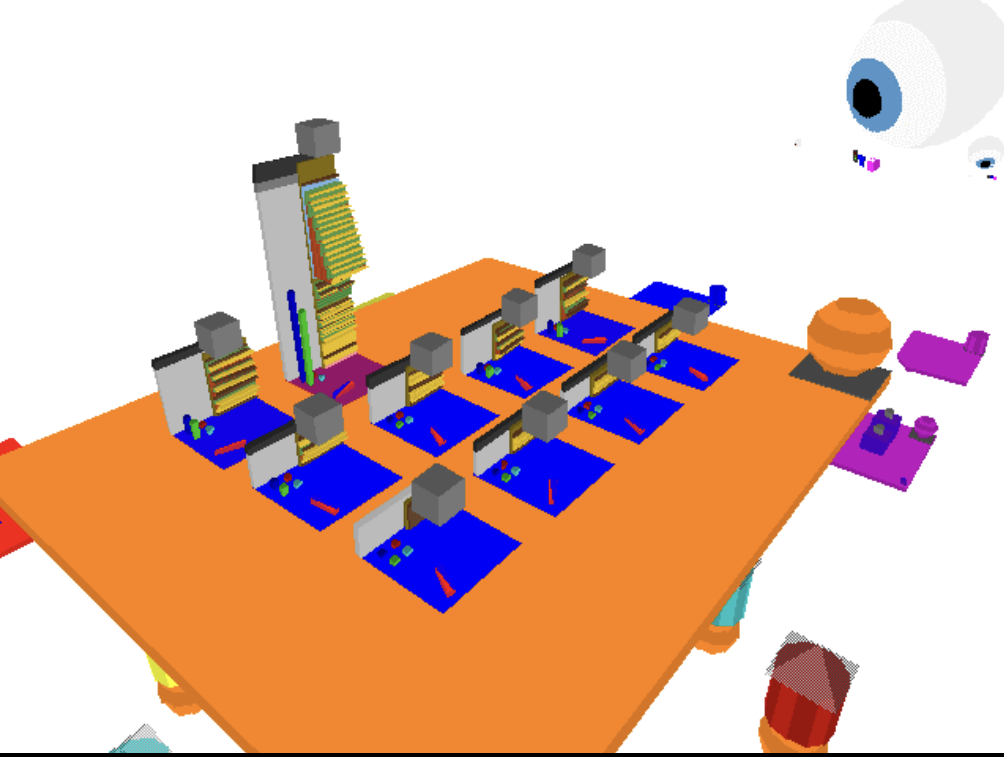
\includegraphics[width=0.5\textwidth]{images/visVRExample.png}
    \caption{Beispiel für eine 3D-Visualisierung von Young und Munro \cite[6]{visSoftwareVR}}
    \label{fig:3DVis}
\end{figure}

Trotzdem können wir auch für unser Ziel der Software-Qualitätsmetrik-Visualisierung Kriterien ableiten, die für eine gute Visualisierung wichtig sind \cite{visSoftwareVR}:
\begin{itemize}
    \item \textbf{Darstellung}: Der wichtigste Aspekt ist die Darstellung der Software. Die Visualisierung sollte die Struktur und den Aufbau der Software verdeutlichen. Die Frage ist also, wie wird die Software dargestellt? 
    \begin{itemize}
        \item Informationsgehalt: Die Visualisierung sollte so viele Informationen wie möglich enthalten.
        \item Niedrige visuelle Komplexität: Als Gegenspieler zum Informationsgehalt steht die visuelle Komplexität. Die Visualisierung sollte so einfach wie möglich gehalten werden, um den Betrachter nicht zu überfordern.
        \item Skalierbarkeit: Die Visualisierung sollte auch bei großen Software-Systemen noch gut lesbar sein. Dies ist besonders wichtig, da wir hier über große Software-Systeme sprechen. Die Autoren von \textit{Visualising Software in virtual reality} \cite{visSoftwareVR} sagen zudem, dass mechanismen Nötig sind, um Komplexität und Informationsgehalt zu steuern und je nach Software-System anpassen zu können.
        \item Stabilität gegenüber Änderungen: Die Visualisierung sollte stabil gegenüber Änderungen in der Software sein. Das bedeutet, dass die Visualisierung sich nur so sehr wie nötig ändert, wenn sich die Software ändert, um eine Versions konsistente Vergleichbarkeit zu ermöglichen und bereits mit der Visualierung vertraute Nutzer nicht zu überfordern.
        \item Gute Visuelle Metaphern: Die Visualisierung sollte gute visuelle Metaphern verwenden, um bereits bekannte Konzepte zu verwenden, um die Software verständlicher zu machen.
    \end{itemize}
    \item \textbf{Abstraktion}: Das Ziel von Visualierung muss sein, unwichtige Details auszublenden und ein verständliches Modell der Software zu erstellen. 
    \item \textbf{Navigation}: Da wir häufig über große Software-Systeme sprechen, kann es schnall passeiren dass Nutzer in der Visualisierung verloren gehen. Es muss also möglich sein, sich gut zurecht zu finden und intuitiv zu wissen, wo was ist, um so ein grfühl für die software zu erhalten.
    \item \textbf{Korrelation mit dem Code}: Die Visualisierung sollte eine gute Korrelation mit dem Code haben. Wenn man die Visualierung sieht, soll man diese auch mit dem Code in Verbindung bringen können. Es sollte also möglich sein, die Visualisierung mit dem Code zu verknüpfen und so ein besseres Verständnis für die Software zu bekommen.
    \item \textbf{Automatisierung}: Die Visualisierung sollte automatisiert werden können - ein Punkt der trivialier weise gegeben ist, da wir hier über algorithmen sprechen, die keine manuelle eingabe benötigen.
\end{itemize}

\subsubsection{CodeCity} \label{sec:CodeCity}


\subsection{Treemap-Layouts} \label{sec:Treemap}

Eine Treemap visualisiert einen Baum, indem jedem Knoten ein Rechteck mit der Fläche A zugewiesen wird, proportional zu seinem zugewiesenen Wert (z.B. Datenmenge oder Marktwert). Nicht-Blatt-Knoten werden dabei üblicherweise durch Rahmen (Container-Rectangles) gekennzeichnet, um die Gruppierung der Kinder zu zeigen. \cite{bruls2000squarified} Die Rechtecke aller Blätter füllen die Fläche des Wurzelrechtecks vollständig aus. Mathematisch entspricht die Eingabedatenstruktur einem gewichteten Baum, bei dem jede Blatteinheit eine numerische Größe hat. Die Fläche eines Eltern-Rechtecks entspricht der Summe der Flächen (Werte) seiner Kinder.

Die konkrete Idee hierarchische DAten in form von Treemaps darzustellen wurde erstmals 1991 von Shneiderman und Johnson \cite{johnson1991tree} vorgestellt. Sie stellten fest, dass die Darstellung von hierarchischen Daten in Form von Bäumen in der Regel nicht sehr anschaulich ist. Sie entwickelten eine Methode, um diese Daten in Form von Rechtecken darzustellen, die die Fläche der Knoten proportional zu ihrem Wert darstellen. Diese Methode wurde als \enquote{Treemap} bezeichnet. Als Ziele dieser Visualierung formulierten sie unter anderem diese Aspekte:
\begin{itemize}
    \item \textbf{Effiziente Nutzung des Platzes:} Generell soll es darum gehen möglichst viele Informationen auf einem kleinen Raum darzustellen.
    \item \textbf{Verständlichkeit:} Die Visualisierung soll so gestaltet sein, dass sie für den Betrachter leicht verständlich ist. Es soll möglich sein schnell und mit nur niedrigem kognitiven Aufwand die dargesllten Informationen zu erfassen.
    \item \textbf{Ästethik:} Die Visualisierung soll ansprechend gestaltet sein.
\end{itemize}

Zuvor bestehende Ansätze zur Visualisierung von hierarchischen Daten waren in der Regel nicht sehr anschaulich, besonders, wenn es um große Datenmengen ging. Listen, Baumdiagramme (siehe Abbildung \ref{fig:baumdiagramm}) oder andere Darstellungen (auch bekannt als Node oder Link-Diagramme) sind nicht in der lage alle diese Aspekte zu erfüllen. Bei Einem typischen Baumdiagram zum Beispiel werden teilweise mehr als die Hälfte der Fläche für Hintergrund genutzt \cite[3]{johnson1991tree} außerdem ist es schwer, außer der Struktur der Daten auch die Metriken darzustellen. Sie kritisieren auch die Darstellung von hierarchischen Daten in Form von Venn-Diagrammen (siehe Abbildung \ref{fig:venndiagram}): \enquote{The space required between regions would certainly preclude this Venn diagram representation from serious consideration for larger structures.}\cite[5]{johnson1991tree} Es ist zwar möglich durch die Größe der Kreise eine Metrik darzustellen, es sei aber nicht möglich eine große Anzahl an Knoten sinnvoll darzustellen. 

\begin{figure}[ht]
    \centering
    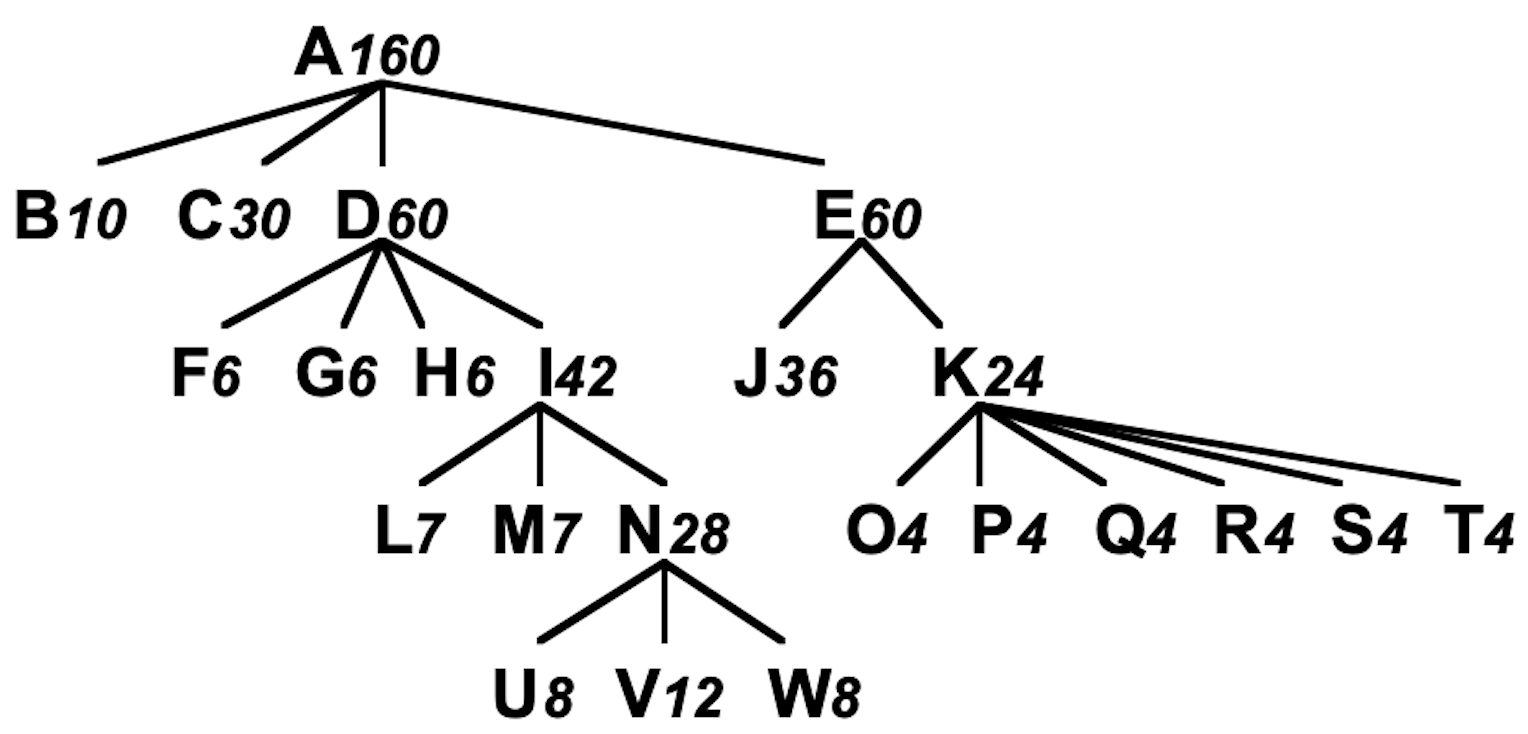
\includegraphics[width=0.5\textwidth]{images/treediagram.png}
    \caption{Beispiel für ein Baumdiagramm}
    \label{fig:baumdiagramm}
\end{figure}

\begin{figure}[ht]
    \centering
    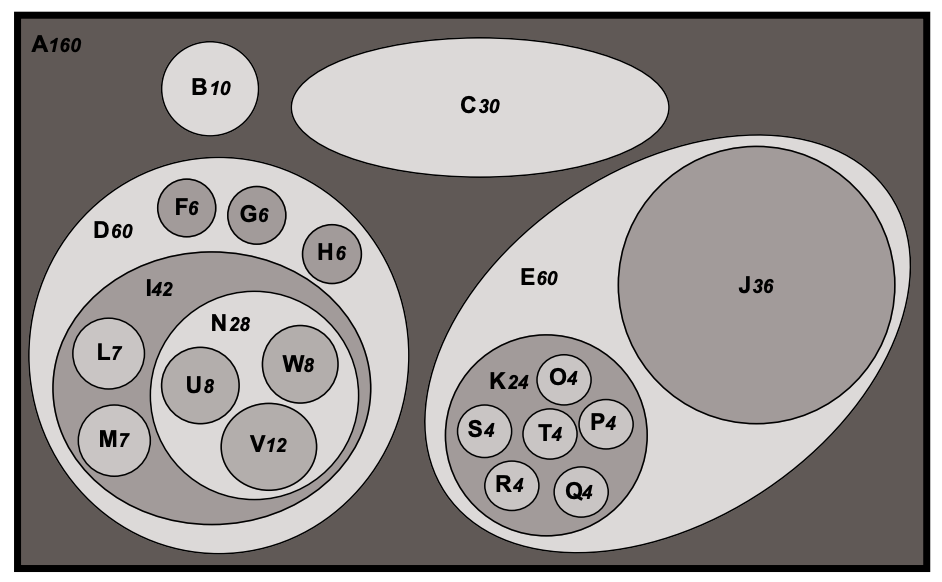
\includegraphics[width=0.5\textwidth]{images/verdiagram.png}
    \caption{Beispiel für ein Venn-Diagramm}
    \label{fig:venndiagram}
\end{figure}

\enquote{Using boxes instead of ovals and a bin-packing algorithm could partially solve this space
problem. But bin-packing is an NP-complete problem and does not preserve order.}\cite[5]{johnson1991tree} Sie stellen fest, dass es theoretisch eine dem Venn Diagramm ähnliche Lösung gibt, die allerdings NP-Hard ist. 

\begin{figure}[ht]
    \centering
    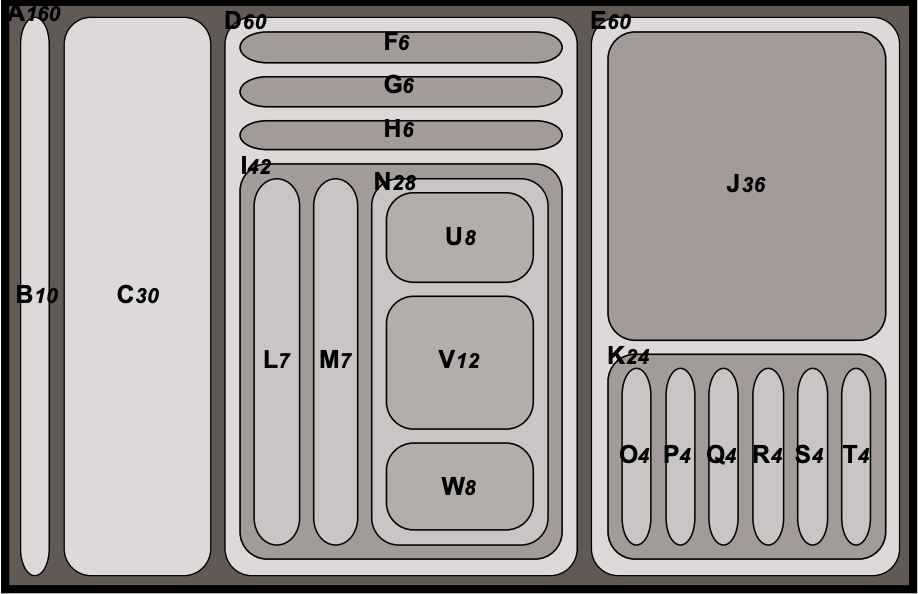
\includegraphics[width=0.5\textwidth]{images/rectVennDiagram.png}
    \caption{Beispiel für ein Boxed Venn-Diagramm}
    \label{fig:rectVennDiagramm}
\end{figure}

Shneiderman und Johnson schlagen zur Lösung dieser Schwierigkeiten ihren Treemap ansatz vor. Sie legen vier Eigenschaften fest, die bei der Erstellung der Treemaps gewährleistet werden:

\begin{itemize}
    \item Wenn ein Knoten 1 ein Vorfahre von Knoten 2 ist, dann ist der Bereich von Knoten 1 vollständig enthalten in dem Bereich von Knoten 2.
    \item Die Bereiche von zwei Knoten schneiden sich, wenn ein Knoten ein Vorfahre des anderen ist.
    \item Knoten belegen eine Fläche, die streng proportional zu ihrem Gewicht ist.
    \item Das Gewicht eines Knotens ist größer oder gleich der Summe der Gewichte seiner Kinder.
\end{itemize}

Sie stellen auch einen Algorithmus vor, der diese Eigenschaften erfüllen soll. Ein von diesem Algorithmus erzeugtes Layout ist in Abbildung \ref{fig:nestedTreemap} dargestellt. 

\begin{figure}[ht]
    \centering
    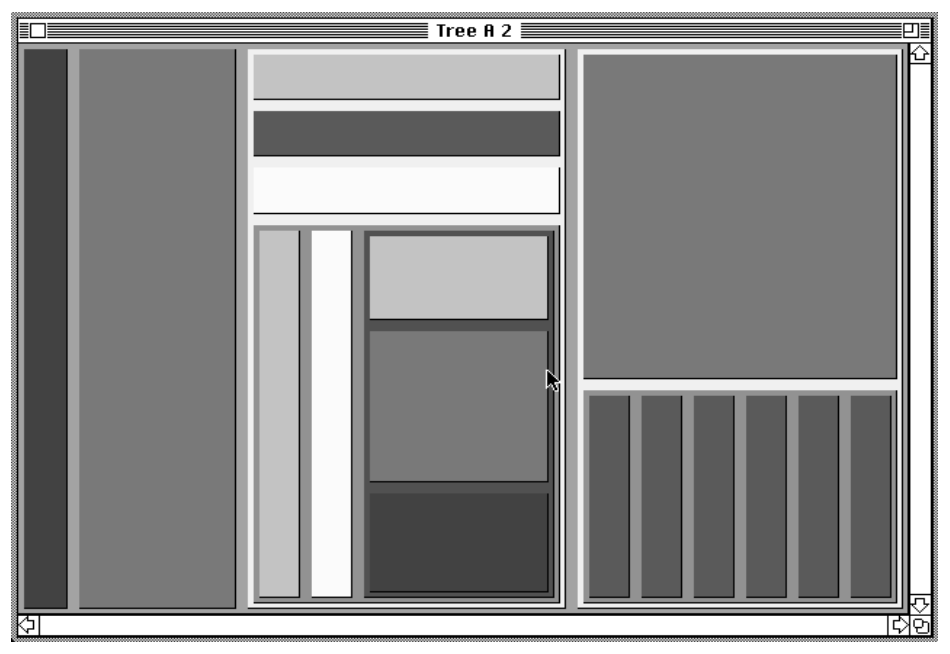
\includegraphics[width=0.5\textwidth]{images/nestedTreemapDiagramm.png}
    \caption{Beispiel für eine Treemap}
    \label{fig:nestedTreemap}
\end{figure}

Der Algorithmus unterteilt den Raum abwechselnd vertikal und horizontal, je nach größe der Knoten. Der Algorithmus arbeitet sich rekursiv von der Wurzel bis zu den Blättern herunter und hat eine Laufzeit von O(n), wobei n die Anzahl der Knoten ist. Im nächsten Abschnitt wird ein ähnlicher Algorithmus im Detail beschrieben, was zum besseren verständis dieser Art von Algorithmen helfen wird.

Obwohl es sich hier um ein renomiertes und viel Zitiertes Paper handelt, machen die Authoren einen entscheidenden Fehler, der in manchen Fällen sogar dazu führen kann, dass Rechtecke komplett verschwinden. Die Authoren betrachten dieses Problem in ihrem Paper leider nicht. 
Der Abstand zwischen den Knoten wird nämlich dadurch erzeugt, dass die Rechtecke diesen Abstand links, recht, oben und unten abgezogen bekommen. Dadurch ist die dargestellte Fläche der Rechtecke nicht mehr proportional zu den Werten, die sie darstellen sollen. Eigenschaft 3 wird also verletzt. Dies ist besonders problematisch, wenn die Rechtecke sehr klein bzw. sehr langgezogen sind. In diesem Fall kann es dazu kommen, dass die Rechtecke so klein werden, dass sie nicht mehr dargestellt werden können. Dies stellt in der Praxis ein riesiges Problem dar, speziell wenn das Problem dieser Arbeit also 3D im kopf bahalten wird. Es kann ja theoretisch vorkommen, dass als Flächenmetrik die lines of code verwendet wird und dort ein file, weil er wenige lines hat sehr klein wird und deswegen aufgrund der margins nicht angezeigt wird. Wenn jetzt aber die metrik für die Höhen berechnung die prozentualle test abdeckung der lines ist und der file nicht getestet ist, dann würde ein potentiell großes problem, was auch eigentlich direkt in auge springen sollte, nicht angezeigt werden. 

Ein weiteres Problem bei diesem Algorithmus ist auch generell, dass unter umständen die Rechtecke sehr langgezogen werden können, was unter Umständen auch Kriterium 3 der Ästethik verletzt. Es gibt viele Ideen dieses Problem anzugehen. Eine Möglichkeit, den Squarify Algorithmus zu verwenden, wird im nöchsten Abschnitt vorgestellt.

\subsubsection{Squarify-Algorithmus} \label{sec:Squarify}

Der Squarify-Algorithmus ist ein Layout-Algorithmus für Treemaps, der darauf abzielt, die Fläche der Rechtecke so ausgewogen wie möglich zu gestalten. Beduetet, dass die Rechtecke möglichst quadratisch sind. Die ursprüngliche form des algorithmusses wurde im Jahr 2000 von Bruls et al. \cite{bruls2000squarified} vorgestellt. Sie stellten fest: \enquote{another problem of standard treemaps [is] the emergence of thin, elongated rectangles}\cite[1]{bruls2000squarified}. wenn rechtecke nicht mehr so langgezogen sind, Es ist einfacher auf Rechtecke zu zeigen, diese wahrzunehmen, sie zu vergleichen und ihre größe einzuschätzen. 

Der Algorithmus arbeitet rekursiv und teilt die Fläche in Rechtecke auf, wobei er versucht, die Seitenverhältnisse der Rechtecke so nah wie möglich an 1 zu halten. Sie stellen einen rekursiven Ansatz vor, bei dem, wie auch bei den meisten anderen Treemap-Algorithmen, die Rechtecke von oben nach unten (also vom Wurzelknoten bis zu den Blattknoten) aufgeteilt werden.

Im Folgenden wird der Algorithmus beschrieben, da er eine wichtige Grundlage für das Verständnis des Problems darstellt und außerdem eine gute Grundlage zum Verständnis der anderen Algorithmen bietet, da viele Algorithmen ähnliche Ideen verwenden.

Der Algorithmus wird anhand eines Beispiels aus dem originalen Squarify-Paper \cite[5]{bruls2000squarified} erläutert. Wir werden den Algorithmus jedoch anders erklären als im Paper, da wir uns näher an der Implementierung orientieren, wie sie in der bekannten d3-Bibliothek \cite{d3_treemap_code} umgesetzt ist.
Es sollen Rechtecke mit den Größen 6, 6, 4, 3, 2, 2, 1 in ein 6 mal 4 Rechteck einsortiert werden.

Der algorithmus arbeitet immer in Reihen, die er versucht zu füllen und dabei die Rechtecke möglichst quadratisch zu halten. Das erste Rechteck ist breiter als lang. (In dieser Arbeit werden wir, anders als in den herkömmlichen papern zu layout algorithmen, das Wort breit als x koordinate und das wort lang als y koordinate nutzen - das hat den hintergrund, dass das wort hoch im drei dimensionalen meist für die z komponent genutzt wird und es sonst zu verwirrungen kommen könnte)
Da das Rechteck in das wir einfügen breiter als lang ist, werden wir eine imaginäre horizontale Reihe so lange mit Rechtecken befüllen, bis ein Threshold erreicht ist. Das erste Rechteck mit größe 6 fügen wir also in Schritt 1 in diese Reihe ein. Das Seitenverhältnis dieses Rechtecks beträgt 8 zu 3 (das Rechteck ist 1.5 Einheiten breit und 4 Einheiten lang). Das zweite Rechteck mit größe 6 fügen wir in Schritt 2 in diese horizontale Reihe ein, dabei wird die Reihe entsprechend breiter. Das Seitenverhältnis des jetzt eingefügten Rechecks beträgt 3 zu 2 (das Rechteck ist 3 Einheiten breit und 2 Einheiten lang). Jetzt kommt das nächste Rechteck mit größe 4. Dieses Rechteck ist hat ein Seitenverhältnis von 4 zu 1 (das Rechteck ist 4 Einheiten breit und 1 Einheit lang). Das hinzufügen dieses Rechtecks führt nun aber dazu, dass das schlechteste Seitenverhältnis der Reihe von 3 zu 2 auf 4 zu 1 ansteigt. Deshalb wird diese Reihe als abgeschlossen angesehen und die nächste Reihe wird begonnen - Schritt 4. 

Dieser Schritt des suchens des schlechtesten Seitenverhältnisses lässt sich von der rechenkomplexität her gut optimieren, sodass der Ratio berechnet werden kann, ohne dass die Reihe wirklich mit Rechtecken gefüllt werden muss. 
Anstatt für jeder Rechteck max(w/l, l/w) zu berechnen, ziehen wir folgende vereinfachung heran.

\begin{align}
    \frac{w_i}{l_i} 
    &= \frac{w_i \cdot l_i \cdot w^2}{l_i \cdot l_i \cdot w^2} \\
    &= \frac{w_i \cdot l_i \cdot w^2}{l_i^2 \cdot \left(\sum_{j=0}^{n} w_j\right)^2} \\
    &= \frac{w_i \cdot l_i \cdot w^2}{\left(l_i \cdot \sum_{j=0}^{n} w_j\right)^2} \\
    &= \frac{w_i \cdot l_i \cdot w^2}{\left(\sum_{j=0}^{n} l_i \cdot w_j\right)^2} \\
    &= \frac{w_i \cdot l_i \cdot w^2}{\left(\sum_{j=0}^{n} l_j \cdot w_j\right)^2}
    \quad\text{da } \forall i, j \in \{0, \dots, n\}, l_i = l_j \\
    &= \frac{V_i \cdot w^2}{sV^2}
\end{align}
Analog dazu gilt das gleich auch für $ \frac{l_i}{w_i} = \frac{sV^2}{V_i \cdot w^2} $. Da wir nur an dem maximalen Wert beider Ausdrücke interessiert sind und die Länge ($l_i$) aller Rechtecke in der Reihe gleich ist, reicht es den Wert für das größte und das kleinste Rechteck zu berechnen und davon den maximalen Wert zu nehmen.

$w$ ist für den gesamten Zeitraum des füllens einer Reihe konstant und muss daher nur einmal berechnet werden. $sV$ wird mit jedem Rechteck aktualisiert. 

Das Ziel ist es das Verhältnis der Seitenlängen gleich zu halten. Im ursprünglichen Paper von Bruls et al. \cite{bruls2000squarified} wird darauf noch nicht so eingegangen, aber viele implementierungen z.b. die von d3.js \cite{d3_treemap_code} ermöglichen es, das Verhältnis nicht nur an den Wert 1 anzunähern, sondern auch an andere Werte, zum Beispiel den goldenen Schnitt. 

\begin{figure}[h]
    \centering
    
\includegraphics[width=0.5\textwidth]{images/oneSquarify.png}
    \caption{Beispiel für ein Squarify-Layout mit Annäherung an quadratische Rechtecke (Durchschnittliches Seitenverhältnis 1.42)}
    \label{fig:squarifyRatio1}
\end{figure}

\begin{figure}[h]
    \centering
    
\includegraphics[width=0.5\textwidth]{images/fiveSquarify.png}
    \caption{Beispiel für ein Squarify-Layout mit Annäherung an den Wert 5 (Durchschnittliches Seitenverhältnis 2.79)}
    \label{fig:squarifyRatio5}
\end{figure}

%wie wirkt sich die reihenfolge auf das layout aus?
\section{Problemstellung} \label{sec:Problemstellung}

Obwohl bereits leistungsfähige Werkzeuge zur Visualisierung existieren, stehen wir vor
zentralen Herausforderungen bei der Darstellung von Codequalitätsmetriken:
• Aussagekraft: Wie lässt sich die Aussagekraft einer Visualisierung erhöhen? Wie
viele Metriken können simultan dargestellt werden?
• Übersichtlichkeit: Wie lässt sich die Übersichtlichkeit der Darstellung erhöhen?
Ermöglicht sie eine gezielte Erkennung individueller Qualitätsprobleme? Ist eine
schnelle Erfassung der Inhalte ohne umfangreiches Vorwissen und Zeitaufwand
möglich?
• Skalierbarkeit: Wie lassen sich umfangreiche Codebasen effektiv visualisieren,
ohne an Übersichtlichkeit einzubüßen? Wie schnell können diese
Visualisierungen generiert werden?

Zielsetzung
Das Ziel dieser Arbeit ist es, Anforderungen an eine effektive Visualisierung von
Codequalitätsmetriken zu definieren und zu zeigen, ob eine verbesserte
Darstellungsmethode existiert.



----------
Was ist uns maibornwolff wichtig bei dem layout?


Christian Hühn gespräch:
Eine Sortierung innerhalb der Ordner ist nicht so wichtig, da die Sortierung eigentlich schon über die ordner struktur hergestellt wird. Außerdem nach was, es macht das bild nicht wirklich übersichtlicher

Kohäsion: entweder gut strukturiert oder schlecht - dann bringt das eh nichts



Ziel ist es schnell und einfach Hotspots zu finden:
Code Charta ist die ausgangslage um die größten Hotspots zu finden

Geredet wird meistens mit Entwicklern

CodeCharta hilft systeme schnell zu verstehen und wo man hinschauen muss
Schnell einen Überblick verschaffen und CodeBasis greifbar machen

Durch 3D mehr verbindungen herstellen: Zb sind große Gebäude auch gut gecovert



Software entwickler nutzen für die analyse selbst erstmal 
Selbst entwickler geben gutes Feedback


Streemap ist nicht so intuitiv - Vorteile sind, dass es sehr stabil ist




Kunden zeigen wie sich ein Projekt geändert hat:
Bei modernisierungs Projekten 
Ansonsten bleibt in audits die basisfläche gleich, somit ist das nicht so wichtig

DD-Audits: 
Screenshots von ein paar Ansichten
Sprechen über hotspots

Software Health-Check
Kunde hat system, was ist da nicht rund?

Code Quality Insights
Screenshots generieren


----

moment mal: ich will eigentlich nur dass die kind knoten ein gutes Seitenverhältnis haben, der rest kann mir ja eigentlich egal sein - oder zumindest nicht so wichtig


\subsection{Das Treemap Problem} \label{sec:TreemapProblem}
In Abschnnit \ref{sec:Treemap} wurde aufgezeigt, dass bereits der initiale Algorithmus von Johnson und Shneiderman \cite{johnson1991tree} ein fundamentales Problem aufweist, wenn Treemaps mit Abständen zwischen Knoten dargestellt werden sollen. 
\begin{itemize}
    \item Da der Abstand von der Fläche der Knoten abgezogen wird, ist die dargestellte Fläche nicht mehr proportional zum Wert des Knotens.
    \item Durch das Abziehen der Abstände kann es passieren, dass Knoten verschwinden, wenn entweder die Länge oder die Breite der Knoten kleiner oder gleich dem Abstand ist.
\end{itemize}


%*************************************************************************
% Recommendations
%*************************************************************************
%\part{Empfehlungen zur Erstellung wissenschaftlicher Abschlussarbeiten}
%\label{pt:recommendations}
%*************************************************************************
% Backmatter
%*************************************************************************
\appendix
%\renewcommand{\thechapter}{\alph{chapter}}
\cleardoublepage
\part{Appendix}
%\include{chapters/examples/appendix01}
%\include{chapters/examples/appendix02}
%*************************************************************************
% Other Stuff in the Back
%*************************************************************************
\cleardoublepage%********************************************************************
% Bibliography
%*******************************************************
% work-around to have small caps also here in the headline
% https://tex.stackexchange.com/questions/188126/wrong-header-in-bibliography-classicthesis
% Thanks to Enrico Gregorio
\defbibheading{bibintoc}[\bibname]{%
  \phantomsection
  \manualmark
  \markboth{\spacedlowsmallcaps{#1}}{\spacedlowsmallcaps{#1}}%
  \addtocontents{toc}{\protect\vspace{\beforebibskip}}%
  \addcontentsline{toc}{chapter}{\tocEntry{#1}}%
  \chapter*{#1}%
}

% allow Linebreaks in urls anywhere
\setcounter{biburlnumpenalty}{100}
\setcounter{biburlucpenalty}{100}
\setcounter{biburllcpenalty}{100}
% enable to long words to break anywhere by increasing the allowed whitespace between words.
\sloppy

\printbibliography[heading=bibintoc]

%*************************************************************************
% Game Over: Restore, Restart, or Quit?
%*************************************************************************
\end{document}
%*************************************************************************
